\documentclass[1p]{elsarticle_modified}
%\bibliographystyle{elsarticle-num}

%\usepackage[colorlinks]{hyperref}
%\usepackage{abbrmath_seonhwa} %\Abb, \Ascr, \Acal ,\Abf, \Afrak
\usepackage{amsfonts}
\usepackage{amssymb}
\usepackage{amsmath}
\usepackage{amsthm}
\usepackage{scalefnt}
\usepackage{amsbsy}
\usepackage{kotex}
\usepackage{caption}
\usepackage{subfig}
\usepackage{color}
\usepackage{graphicx}
\usepackage{xcolor} %% white, black, red, green, blue, cyan, magenta, yellow
\usepackage{float}
\usepackage{setspace}
\usepackage{hyperref}

\usepackage{tikz}
\usetikzlibrary{arrows}

\usepackage{multirow}
\usepackage{array} % fixed length table
\usepackage{hhline}

%%%%%%%%%%%%%%%%%%%%%
\makeatletter
\renewcommand*\env@matrix[1][\arraystretch]{%
	\edef\arraystretch{#1}%
	\hskip -\arraycolsep
	\let\@ifnextchar\new@ifnextchar
	\array{*\c@MaxMatrixCols c}}
\makeatother %https://tex.stackexchange.com/questions/14071/how-can-i-increase-the-line-spacing-in-a-matrix
%%%%%%%%%%%%%%%

\usepackage[normalem]{ulem}

\newcommand{\msout}[1]{\ifmmode\text{\sout{\ensuremath{#1}}}\else\sout{#1}\fi}
%SOURCE: \msout is \stkout macro in https://tex.stackexchange.com/questions/20609/strikeout-in-math-mode

\newcommand{\cancel}[1]{
	\ifmmode
	{\color{red}\msout{#1}}
	\else
	{\color{red}\sout{#1}}
	\fi
}

\newcommand{\add}[1]{
	{\color{blue}\uwave{#1}}
}

\newcommand{\replace}[2]{
	\ifmmode
	{\color{red}\msout{#1}}{\color{blue}\uwave{#2}}
	\else
	{\color{red}\sout{#1}}{\color{blue}\uwave{#2}}
	\fi
}

\newcommand{\Sol}{\mathcal{S}} %segment
\newcommand{\D}{D} %diagram
\newcommand{\A}{\mathcal{A}} %arc


%%%%%%%%%%%%%%%%%%%%%%%%%%%%%5 test

\def\sl{\operatorname{\textup{SL}}(2,\Cbb)}
\def\psl{\operatorname{\textup{PSL}}(2,\Cbb)}
\def\quan{\mkern 1mu \triangleright \mkern 1mu}

\theoremstyle{definition}
\newtheorem{thm}{Theorem}[section]
\newtheorem{prop}[thm]{Proposition}
\newtheorem{lem}[thm]{Lemma}
\newtheorem{ques}[thm]{Question}
\newtheorem{cor}[thm]{Corollary}
\newtheorem{defn}[thm]{Definition}
\newtheorem{exam}[thm]{Example}
\newtheorem{rmk}[thm]{Remark}
\newtheorem{alg}[thm]{Algorithm}

\newcommand{\I}{\sqrt{-1}}
\begin{document}

%\begin{frontmatter}
%
%\title{Boundary parabolic representations of knots up to 8 crossings}
%
%%% Group authors per affiliation:
%\author{Yunhi Cho} 
%\address{Department of Mathematics, University of Seoul, Seoul, Korea}
%\ead{yhcho@uos.ac.kr}
%
%
%\author{Seonhwa Kim} %\fnref{s_kim}}
%\address{Center for Geometry and Physics, Institute for Basic Science, Pohang, 37673, Korea}
%\ead{ryeona17@ibs.re.kr}
%
%\author{Hyuk Kim}
%\address{Department of Mathematical Sciences, Seoul National University, Seoul 08826, Korea}
%\ead{hyukkim@snu.ac.kr}
%
%\author{Seokbeom Yoon}
%\address{Department of Mathematical Sciences, Seoul National University, Seoul, 08826,  Korea}
%\ead{sbyoon15@snu.ac.kr}
%
%\begin{abstract}
%We find all boundary parabolic representation of knots up to 8 crossings.
%
%\end{abstract}
%\begin{keyword}
%    \MSC[2010] 57M25 
%\end{keyword}
%
%\end{frontmatter}

%\linenumbers
%\tableofcontents
%
\newcommand\colored[1]{\textcolor{white}{\rule[-0.35ex]{0.8em}{1.4ex}}\kern-0.8em\color{red} #1}%
%\newcommand\colored[1]{\textcolor{white}{ #1}\kern-2.17ex	\textcolor{white}{ #1}\kern-1.81ex	\textcolor{white}{ #1}\kern-2.15ex\color{red}#1	}

{\Large $\underline{12n_{0664}~(K12n_{0664})}$}

\setlength{\tabcolsep}{10pt}
\renewcommand{\arraystretch}{1.6}
\vspace{1cm}\begin{tabular}{m{100pt}>{\centering\arraybackslash}m{274pt}}
\multirow{5}{120pt}{
	\centering
	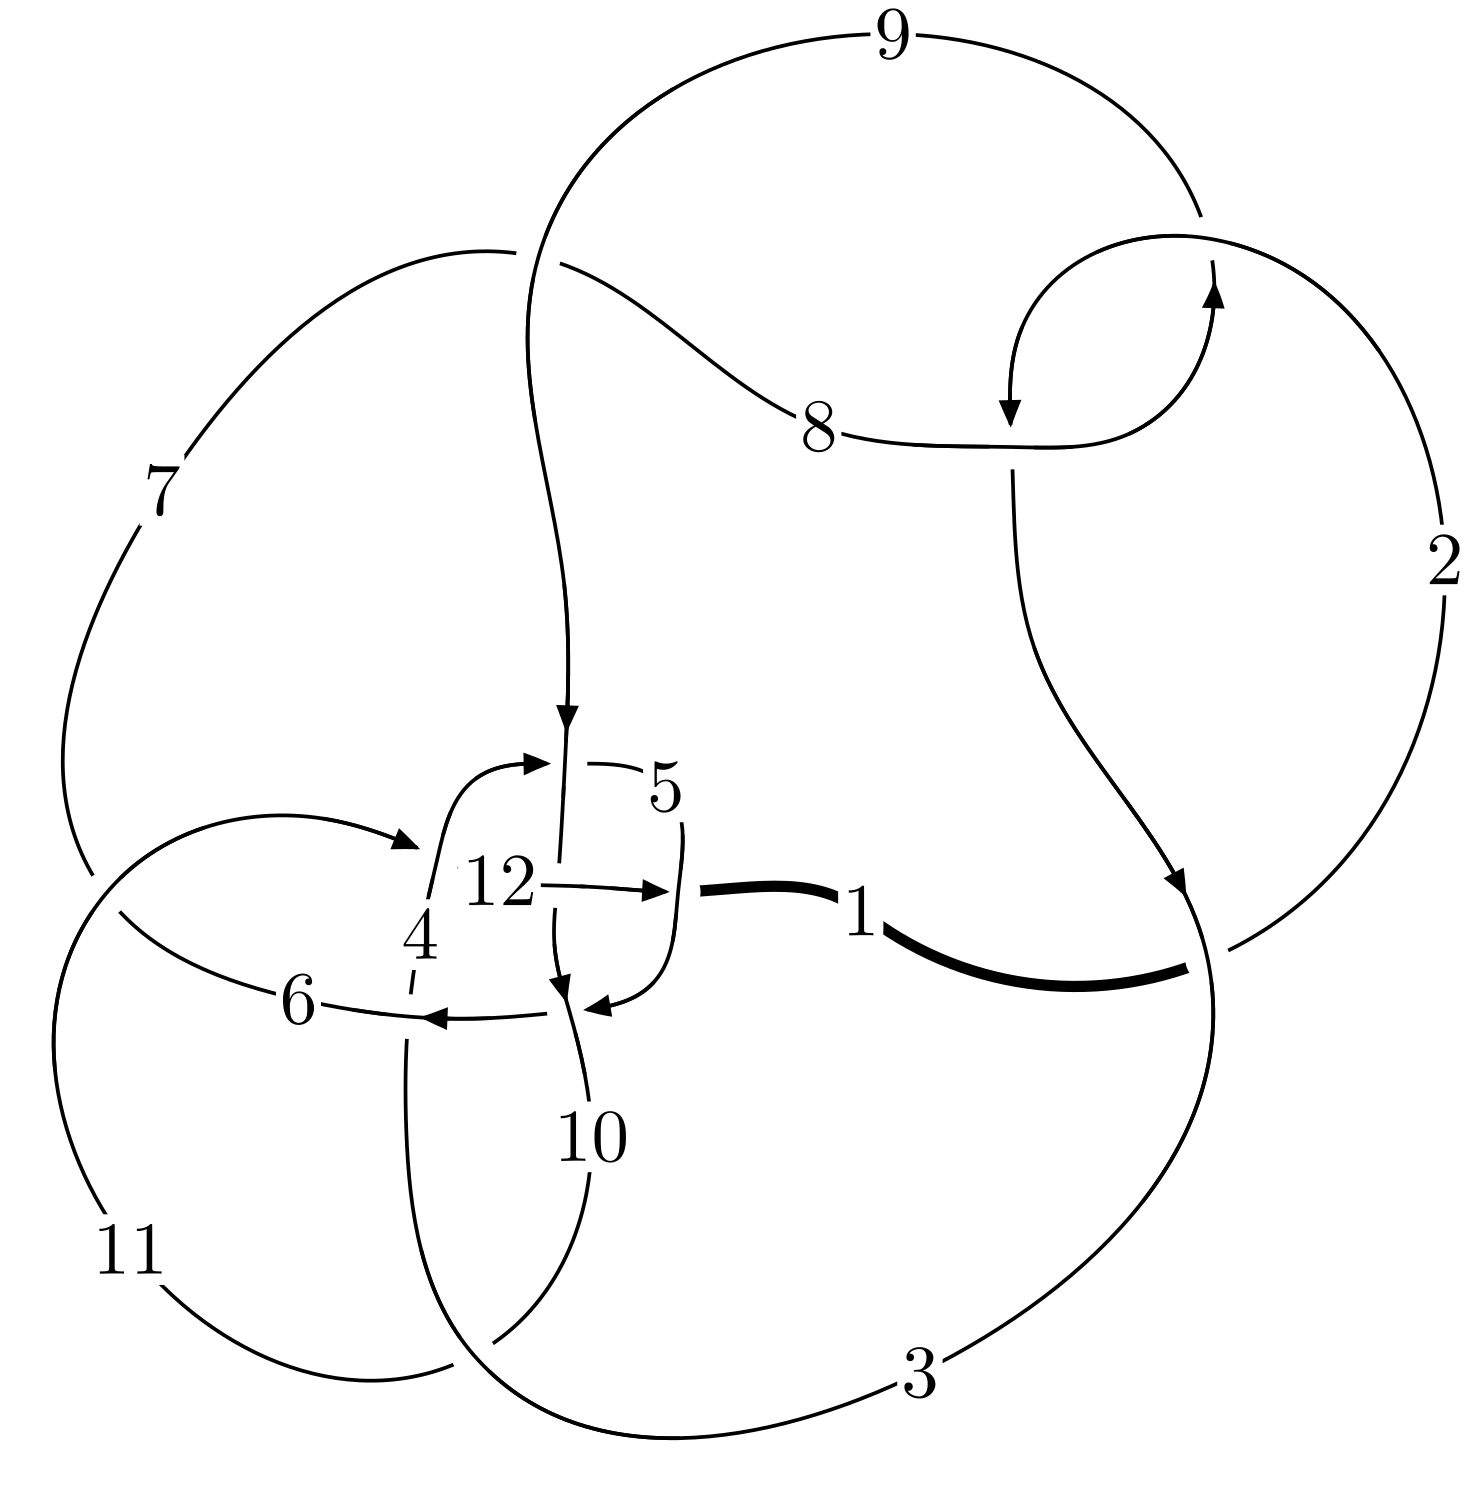
\includegraphics[width=112pt]{../../../GIT/diagram.site/Diagrams/png/2753_12n_0664.png}\\
\ \ \ A knot diagram\footnotemark}&
\allowdisplaybreaks
\textbf{Linearized knot diagam} \\
\cline{2-2}
 &
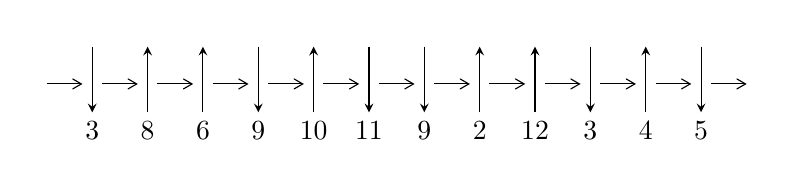
\begin{tikzpicture}[x=20pt, y=17pt]
	% nodes
	\node (C0) at (0, 0) {};
	\node (C1) at (1, 0) {};
	\node (C1U) at (1, +1) {};
	\node (C1D) at (1, -1) {3};

	\node (C2) at (2, 0) {};
	\node (C2U) at (2, +1) {};
	\node (C2D) at (2, -1) {8};

	\node (C3) at (3, 0) {};
	\node (C3U) at (3, +1) {};
	\node (C3D) at (3, -1) {6};

	\node (C4) at (4, 0) {};
	\node (C4U) at (4, +1) {};
	\node (C4D) at (4, -1) {9};

	\node (C5) at (5, 0) {};
	\node (C5U) at (5, +1) {};
	\node (C5D) at (5, -1) {10};

	\node (C6) at (6, 0) {};
	\node (C6U) at (6, +1) {};
	\node (C6D) at (6, -1) {11};

	\node (C7) at (7, 0) {};
	\node (C7U) at (7, +1) {};
	\node (C7D) at (7, -1) {9};

	\node (C8) at (8, 0) {};
	\node (C8U) at (8, +1) {};
	\node (C8D) at (8, -1) {2};

	\node (C9) at (9, 0) {};
	\node (C9U) at (9, +1) {};
	\node (C9D) at (9, -1) {12};

	\node (C10) at (10, 0) {};
	\node (C10U) at (10, +1) {};
	\node (C10D) at (10, -1) {3};

	\node (C11) at (11, 0) {};
	\node (C11U) at (11, +1) {};
	\node (C11D) at (11, -1) {4};

	\node (C12) at (12, 0) {};
	\node (C12U) at (12, +1) {};
	\node (C12D) at (12, -1) {5};
	\node (C13) at (13, 0) {};

	% arrows
	\draw[->,>={angle 60}]
	(C0) edge (C1) (C1) edge (C2) (C2) edge (C3) (C3) edge (C4) (C4) edge (C5) (C5) edge (C6) (C6) edge (C7) (C7) edge (C8) (C8) edge (C9) (C9) edge (C10) (C10) edge (C11) (C11) edge (C12) (C12) edge (C13) ;	\draw[->,>=stealth]
	(C1U) edge (C1D) (C2D) edge (C2U) (C3D) edge (C3U) (C4U) edge (C4D) (C5D) edge (C5U) (C6U) edge (C6D) (C7U) edge (C7D) (C8D) edge (C8U) (C9D) edge (C9U) (C10U) edge (C10D) (C11D) edge (C11U) (C12U) edge (C12D) ;
	\end{tikzpicture} \\
\hhline{~~} \\& 
\textbf{Solving Sequence} \\ \cline{2-2} 
 &
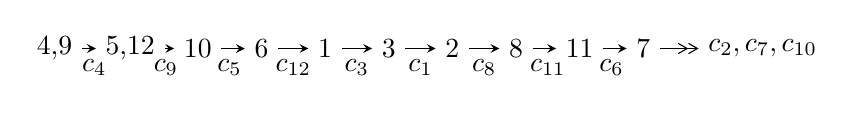
\begin{tikzpicture}[x=23pt, y=7pt]
	% node
	\node (A0) at (-1/8, 0) {4,9};
	\node (A1) at (17/16, 0) {5,12};
	\node (A2) at (17/8, 0) {10};
	\node (A3) at (25/8, 0) {6};
	\node (A4) at (33/8, 0) {1};
	\node (A5) at (41/8, 0) {3};
	\node (A6) at (49/8, 0) {2};
	\node (A7) at (57/8, 0) {8};
	\node (A8) at (65/8, 0) {11};
	\node (A9) at (73/8, 0) {7};
	\node (C1) at (1/2, -1) {$c_{4}$};
	\node (C2) at (13/8, -1) {$c_{9}$};
	\node (C3) at (21/8, -1) {$c_{5}$};
	\node (C4) at (29/8, -1) {$c_{12}$};
	\node (C5) at (37/8, -1) {$c_{3}$};
	\node (C6) at (45/8, -1) {$c_{1}$};
	\node (C7) at (53/8, -1) {$c_{8}$};
	\node (C8) at (61/8, -1) {$c_{11}$};
	\node (C9) at (69/8, -1) {$c_{6}$};
	\node (A10) at (11, 0) {$c_{2},c_{7},c_{10}$};

	% edge
	\draw[->,>=stealth]	
	(A0) edge (A1) (A1) edge (A2) (A2) edge (A3) (A3) edge (A4) (A4) edge (A5) (A5) edge (A6) (A6) edge (A7) (A7) edge (A8) (A8) edge (A9) ;
	\draw[->>,>={angle 60}]	
	(A9) edge (A10);
\end{tikzpicture} \\ 

\end{tabular} \\

\footnotetext{
The image of knot diagram is generated by the software ``\textbf{Draw programme}" developed by Andrew Bartholomew(\url{http://www.layer8.co.uk/maths/draw/index.htm\#Running-draw}), where we modified some parts for our purpose(\url{https://github.com/CATsTAILs/LinksPainter}).
}\phantom \\ \newline 
\centering \textbf{Ideals for irreducible components\footnotemark of $X_{\text{par}}$} 
 
\begin{align*}
I^u_{1}&=\langle 
74009148936 u^{22}-76652535715 u^{21}+\cdots+605037775238 b-84815080599,\\
\phantom{I^u_{1}}&\phantom{= \langle  }2192438106671 u^{22}-2107623026072 u^{21}+\cdots+605037775238 a-2052230519656,\\
\phantom{I^u_{1}}&\phantom{= \langle  }u^{23}- u^{22}+\cdots- u+1\rangle \\
I^u_{2}&=\langle 
-1.45654\times10^{19} u^{19}+6.73104\times10^{18} u^{18}+\cdots+1.62289\times10^{20} b-2.33528\times10^{19},\\
\phantom{I^u_{2}}&\phantom{= \langle  }3.70637\times10^{20} u^{19}+2.33528\times10^{19} u^{18}+\cdots+1.62289\times10^{20} a+1.58962\times10^{21},\;u^{20}- u^{18}+\cdots+3 u+1\rangle \\
I^u_{3}&=\langle 
1.59937\times10^{20} u^{19}+2.00847\times10^{20} u^{18}+\cdots+2.29962\times10^{21} b+5.16126\times10^{21},\\
\phantom{I^u_{3}}&\phantom{= \langle  }191496437465195 u^{19}+59872033526663 u^{18}+\cdots+4748609612427635 a+5069797018706783,\\
\phantom{I^u_{3}}&\phantom{= \langle  }u^{20}+u^{19}+\cdots-30 u+25\rangle \\
I^u_{4}&=\langle 
-4.98032\times10^{100} u^{39}+3.96797\times10^{100} u^{38}+\cdots+8.14259\times10^{103} b+9.25727\times10^{103},\\
\phantom{I^u_{4}}&\phantom{= \langle  }-6.53696\times10^{86} u^{39}+5.50591\times10^{86} u^{38}+\cdots+6.14311\times10^{89} a+9.18988\times10^{89},\\
\phantom{I^u_{4}}&\phantom{= \langle  }u^{40}- u^{39}+\cdots-2058 u+661\rangle \\
I^u_{5}&=\langle 
-9.70252\times10^{33} u^{33}-1.36400\times10^{34} u^{32}+\cdots+2.93977\times10^{34} b+1.13426\times10^{34},\\
\phantom{I^u_{5}}&\phantom{= \langle  }3.22079\times10^{34} u^{33}+2.08653\times10^{34} u^{32}+\cdots+2.93977\times10^{34} a-8.32299\times10^{34},\;u^{34}+u^{33}+\cdots- u+1\rangle \\
I^u_{6}&=\langle 
b- u,\;a,\;u^5+u^4-2 u^3- u^2+u-1\rangle \\
I^u_{7}&=\langle 
2405 u^9-2260 u^8+\cdots+7829 b-605,\;- u^9+u^8+2 u^7+2 u^6+2 u^5-12 u^4-9 u^3-9 u^2+a-6 u,\\
\phantom{I^u_{7}}&\phantom{= \langle  }u^{10}- u^9-2 u^8-2 u^7-2 u^6+12 u^5+9 u^4+9 u^3+6 u^2-1\rangle \\
I^u_{8}&=\langle 
b+u-1,\;a+u,\;u^2- u+1\rangle \\
\\
\end{align*}
\raggedright * 8 irreducible components of $\dim_{\mathbb{C}}=0$, with total 154 representations.\\
\footnotetext{All coefficients of polynomials are rational numbers. But the coefficients are sometimes approximated in decimal forms when there is not enough margin.}
\newpage
\renewcommand{\arraystretch}{1}
\centering \section*{I. $I^u_{1}= \langle 7.40\times10^{10} u^{22}-7.67\times10^{10} u^{21}+\cdots+6.05\times10^{11} b-8.48\times10^{10},\;2.19\times10^{12} u^{22}-2.11\times10^{12} u^{21}+\cdots+6.05\times10^{11} a-2.05\times10^{12},\;u^{23}- u^{22}+\cdots- u+1 \rangle$}
\flushleft \textbf{(i) Arc colorings}\\
\begin{tabular}{m{7pt} m{180pt} m{7pt} m{180pt} }
\flushright $a_{4}=$&$\begin{pmatrix}1\\0\end{pmatrix}$ \\
\flushright $a_{9}=$&$\begin{pmatrix}0\\u\end{pmatrix}$ \\
\flushright $a_{5}=$&$\begin{pmatrix}1\\u^2\end{pmatrix}$ \\
\flushright $a_{12}=$&$\begin{pmatrix}-3.62364 u^{22}+3.48346 u^{21}+\cdots+36.4991 u+3.39190\\-0.122322 u^{22}+0.126690 u^{21}+\cdots+4.48346 u+0.140181\end{pmatrix}$ \\
\flushright $a_{10}=$&$\begin{pmatrix}-8.75272 u^{22}+8.03309 u^{21}+\cdots+60.0017 u+7.21619\\-0.877678 u^{22}+0.873310 u^{21}+\cdots+12.5165 u+0.859819\end{pmatrix}$ \\
\flushright $a_{6}=$&$\begin{pmatrix}2.39190 u^{22}+0.231734 u^{21}+\cdots+7.02051 u-22.8910\\0.140181 u^{22}-0.0178599 u^{21}+\cdots+0.231734 u-3.62364\end{pmatrix}$ \\
\flushright $a_{1}=$&$\begin{pmatrix}-3.62364 u^{22}+3.48346 u^{21}+\cdots+35.4991 u+3.39190\\-0.122322 u^{22}+0.126690 u^{21}+\cdots+4.48346 u+0.140181\end{pmatrix}$ \\
\flushright $a_{3}=$&$\begin{pmatrix}-3.96447 u^{22}-1.28694 u^{21}+\cdots-19.1702 u+31.9505\\-0.719637 u^{22}-0.0357199 u^{21}+\cdots-1.53653 u+8.75272\end{pmatrix}$ \\
\flushright $a_{2}=$&$\begin{pmatrix}-2.70321 u^{22}+3.47564 u^{21}+\cdots+3.10966 u-15.1028\\-5.51731 u^{22}+4.69612 u^{21}+\cdots+18.0155 u+1.76587\end{pmatrix}$ \\
\flushright $a_{8}=$&$\begin{pmatrix}2.24735 u^{22}+0.226332 u^{21}+\cdots+6.77092 u-19.3897\\0.317416 u^{22}-0.0214925 u^{21}+\cdots+0.475926 u-5.97500\end{pmatrix}$ \\
\flushright $a_{11}=$&$\begin{pmatrix}-3.50132 u^{22}+3.35677 u^{21}+\cdots+32.0157 u+3.25172\\-0.122322 u^{22}+0.126690 u^{21}+\cdots+4.48346 u+0.140181\end{pmatrix}$ \\
\flushright $a_{7}=$&$\begin{pmatrix}2.24735 u^{22}+0.226332 u^{21}+\cdots+6.77092 u-19.3897\\0.144550 u^{22}+0.00540143 u^{21}+\cdots+0.249594 u-3.50132\end{pmatrix}$\\&\end{tabular}
\flushleft \textbf{(ii) Obstruction class $= -1$}\\~\\
\flushleft \textbf{(iii) Cusp Shapes $= \frac{7925175549593}{302518887619} u^{22}-\frac{5141352911335}{302518887619} u^{21}+\cdots-\frac{24756789749065}{302518887619} u-\frac{8458236233113}{302518887619}$}\\~\\
\newpage\renewcommand{\arraystretch}{1}
\flushleft \textbf{(iv) u-Polynomials at the component}\newline \\
\begin{tabular}{m{50pt}|m{274pt}}
Crossings & \hspace{64pt}u-Polynomials at each crossing \\
\hline $$\begin{aligned}c_{1},c_{7}\end{aligned}$$&$\begin{aligned}
&u^{23}+10 u^{22}+\cdots+208 u-64
\end{aligned}$\\
\hline $$\begin{aligned}c_{2},c_{8}\end{aligned}$$&$\begin{aligned}
&u^{23}+6 u^{22}+\cdots-28 u-8
\end{aligned}$\\
\hline $$\begin{aligned}c_{3},c_{9}\end{aligned}$$&$\begin{aligned}
&u^{23}+11 u^{22}+\cdots-187 u-49
\end{aligned}$\\
\hline $$\begin{aligned}c_{4},c_{6},c_{10}\\c_{12}\end{aligned}$$&$\begin{aligned}
&u^{23}+u^{22}+\cdots- u-1
\end{aligned}$\\
\hline $$\begin{aligned}c_{5},c_{11}\end{aligned}$$&$\begin{aligned}
&u^{23}-2 u^{22}+\cdots- u-4
\end{aligned}$\\
\hline
\end{tabular}\\~\\
\newpage\renewcommand{\arraystretch}{1}
\flushleft \textbf{(v) Riley Polynomials at the component}\newline \\
\begin{tabular}{m{50pt}|m{274pt}}
Crossings & \hspace{64pt}Riley Polynomials at each crossing \\
\hline $$\begin{aligned}c_{1},c_{7}\end{aligned}$$&$\begin{aligned}
&y^{23}+6 y^{22}+\cdots+153856 y-4096
\end{aligned}$\\
\hline $$\begin{aligned}c_{2},c_{8}\end{aligned}$$&$\begin{aligned}
&y^{23}+10 y^{22}+\cdots+208 y-64
\end{aligned}$\\
\hline $$\begin{aligned}c_{3},c_{9}\end{aligned}$$&$\begin{aligned}
&y^{23}-11 y^{22}+\cdots+9979 y-2401
\end{aligned}$\\
\hline $$\begin{aligned}c_{4},c_{6},c_{10}\\c_{12}\end{aligned}$$&$\begin{aligned}
&y^{23}-19 y^{22}+\cdots+35 y-1
\end{aligned}$\\
\hline $$\begin{aligned}c_{5},c_{11}\end{aligned}$$&$\begin{aligned}
&y^{23}-4 y^{22}+\cdots+81 y-16
\end{aligned}$\\
\hline
\end{tabular}\\~\\
\newpage\flushleft \textbf{(vi) Complex Volumes and Cusp Shapes}
$$\begin{array}{c|c|c}  
\text{Solutions to }I^u_{1}& \I (\text{vol} + \sqrt{-1}CS) & \text{Cusp shape}\\
 \hline 
\begin{aligned}
u &= \phantom{-}1.070790 + 0.187276 I \\
a &= -0.742987 - 0.362569 I \\
b &= \phantom{-}0.390360 - 0.513715 I\end{aligned}
 & -2.83605 - 0.34568 I & -1.92962 - 0.43168 I \\ \hline\begin{aligned}
u &= \phantom{-}1.070790 - 0.187276 I \\
a &= -0.742987 + 0.362569 I \\
b &= \phantom{-}0.390360 + 0.513715 I\end{aligned}
 & -2.83605 + 0.34568 I & -1.92962 + 0.43168 I \\ \hline\begin{aligned}
u &= -1.072600 + 0.407037 I \\
a &= \phantom{-}0.766205 - 0.399094 I \\
b &= -0.666528 - 0.655018 I\end{aligned}
 & -5.89444 + 5.46645 I & -3.61005 - 3.53353 I \\ \hline\begin{aligned}
u &= -1.072600 - 0.407037 I \\
a &= \phantom{-}0.766205 + 0.399094 I \\
b &= -0.666528 + 0.655018 I\end{aligned}
 & -5.89444 - 5.46645 I & -3.61005 + 3.53353 I \\ \hline\begin{aligned}
u &= \phantom{-}1.110920 + 0.398545 I \\
a &= -0.834089 + 0.961871 I \\
b &= -0.637726 + 0.694268 I\end{aligned}
 & \phantom{-}2.55401 - 3.06813 I & -1.63871 + 4.65576 I \\ \hline\begin{aligned}
u &= \phantom{-}1.110920 - 0.398545 I \\
a &= -0.834089 - 0.961871 I \\
b &= -0.637726 - 0.694268 I\end{aligned}
 & \phantom{-}2.55401 + 3.06813 I & -1.63871 - 4.65576 I \\ \hline\begin{aligned}
u &= -1.135800 + 0.574185 I \\
a &= \phantom{-}0.605932 + 1.053290 I \\
b &= \phantom{-}0.819929 + 0.795383 I\end{aligned}
 & \phantom{-}2.70586 + 9.35880 I & \phantom{-}0.02921 - 9.42828 I \\ \hline\begin{aligned}
u &= -1.135800 - 0.574185 I \\
a &= \phantom{-}0.605932 - 1.053290 I \\
b &= \phantom{-}0.819929 - 0.795383 I\end{aligned}
 & \phantom{-}2.70586 - 9.35880 I & \phantom{-}0.02921 + 9.42828 I \\ \hline\begin{aligned}
u &= -1.338780 + 0.103629 I \\
a &= \phantom{-}0.734386 - 0.447547 I \\
b &= -0.154582 - 0.897495 I\end{aligned}
 & -7.50009 - 3.86771 I & -5.29636 + 4.05215 I \\ \hline\begin{aligned}
u &= -1.338780 - 0.103629 I \\
a &= \phantom{-}0.734386 + 0.447547 I \\
b &= -0.154582 + 0.897495 I\end{aligned}
 & -7.50009 + 3.86771 I & -5.29636 - 4.05215 I\\
 \hline 
 \end{array}$$\newpage$$\begin{array}{c|c|c}  
\text{Solutions to }I^u_{1}& \I (\text{vol} + \sqrt{-1}CS) & \text{Cusp shape}\\
 \hline 
\begin{aligned}
u &= \phantom{-}0.559367 + 0.131643 I \\
a &= \phantom{-}0.475373 - 0.977519 I \\
b &= \phantom{-}0.843832 - 0.087265 I\end{aligned}
 & -0.89508 - 1.63405 I & -5.04879 + 5.49945 I \\ \hline\begin{aligned}
u &= \phantom{-}0.559367 - 0.131643 I \\
a &= \phantom{-}0.475373 + 0.977519 I \\
b &= \phantom{-}0.843832 + 0.087265 I\end{aligned}
 & -0.89508 + 1.63405 I & -5.04879 - 5.49945 I \\ \hline\begin{aligned}
u &= -0.497228\phantom{ +0.000000I} \\
a &= -1.49813\phantom{ +0.000000I} \\
b &= -0.867620\phantom{ +0.000000I}\end{aligned}
 & \phantom{-}1.46426\phantom{ +0.000000I} & \phantom{-}7.43570\phantom{ +0.000000I} \\ \hline\begin{aligned}
u &= \phantom{-}0.407932 + 0.126673 I \\
a &= \phantom{-}1.76152 - 2.42535 I \\
b &= \phantom{-}0.923455 - 0.055957 I\end{aligned}
 & \phantom{-}3.57163 - 6.00249 I & \phantom{-}1.32822 + 3.13711 I \\ \hline\begin{aligned}
u &= \phantom{-}0.407932 - 0.126673 I \\
a &= \phantom{-}1.76152 + 2.42535 I \\
b &= \phantom{-}0.923455 + 0.055957 I\end{aligned}
 & \phantom{-}3.57163 + 6.00249 I & \phantom{-}1.32822 - 3.13711 I \\ \hline\begin{aligned}
u &= -0.410517 + 0.091700 I \\
a &= -2.27314 - 1.89786 I \\
b &= -0.917370 - 0.041035 I\end{aligned}
 & \phantom{-}4.23594 + 0.53344 I & \phantom{-}5.35636 + 2.56439 I \\ \hline\begin{aligned}
u &= -0.410517 - 0.091700 I \\
a &= -2.27314 + 1.89786 I \\
b &= -0.917370 + 0.041035 I\end{aligned}
 & \phantom{-}4.23594 - 0.53344 I & \phantom{-}5.35636 - 2.56439 I \\ \hline\begin{aligned}
u &= -1.35567 + 1.04234 I \\
a &= \phantom{-}0.196756 + 0.866889 I \\
b &= \phantom{-}1.24211 + 1.13763 I\end{aligned}
 & -1.33962 + 13.52040 I & \phantom{-}1.78577 - 7.19541 I \\ \hline\begin{aligned}
u &= -1.35567 - 1.04234 I \\
a &= \phantom{-}0.196756 - 0.866889 I \\
b &= \phantom{-}1.24211 - 1.13763 I\end{aligned}
 & -1.33962 - 13.52040 I & \phantom{-}1.78577 + 7.19541 I \\ \hline\begin{aligned}
u &= \phantom{-}1.51219 + 0.87780 I \\
a &= -0.303869 + 0.790076 I \\
b &= -1.04602 + 1.26900 I\end{aligned}
 & -6.64500 - 9.40579 I & -3.02964 + 5.28602 I\\
 \hline 
 \end{array}$$\newpage$$\begin{array}{c|c|c}  
\text{Solutions to }I^u_{1}& \I (\text{vol} + \sqrt{-1}CS) & \text{Cusp shape}\\
 \hline 
\begin{aligned}
u &= \phantom{-}1.51219 - 0.87780 I \\
a &= -0.303869 - 0.790076 I \\
b &= -1.04602 - 1.26900 I\end{aligned}
 & -6.64500 + 9.40579 I & -3.02964 - 5.28602 I \\ \hline\begin{aligned}
u &= \phantom{-}1.40078 + 1.17174 I \\
a &= -0.137018 + 0.817530 I \\
b &= -1.36365 + 1.20364 I\end{aligned}
 & -4.3162 - 19.1491 I & \phantom{-0.000000 -}0. + 10.19089 I \\ \hline\begin{aligned}
u &= \phantom{-}1.40078 - 1.17174 I \\
a &= -0.137018 - 0.817530 I \\
b &= -1.36365 - 1.20364 I\end{aligned}
 & -4.3162 + 19.1491 I & \phantom{-0.000000 } 0. - 10.19089 I\\
 \hline 
 \end{array}$$\newpage\newpage\renewcommand{\arraystretch}{1}
\centering \section*{II. $I^u_{2}= \langle -1.46\times10^{19} u^{19}+6.73\times10^{18} u^{18}+\cdots+1.62\times10^{20} b-2.34\times10^{19},\;3.71\times10^{20} u^{19}+2.34\times10^{19} u^{18}+\cdots+1.62\times10^{20} a+1.59\times10^{21},\;u^{20}- u^{18}+\cdots+3 u+1 \rangle$}
\flushleft \textbf{(i) Arc colorings}\\
\begin{tabular}{m{7pt} m{180pt} m{7pt} m{180pt} }
\flushright $a_{4}=$&$\begin{pmatrix}1\\0\end{pmatrix}$ \\
\flushright $a_{9}=$&$\begin{pmatrix}0\\u\end{pmatrix}$ \\
\flushright $a_{5}=$&$\begin{pmatrix}1\\u^2\end{pmatrix}$ \\
\flushright $a_{12}=$&$\begin{pmatrix}-2.28382 u^{19}-0.143897 u^{18}+\cdots-130.160 u-9.79501\\0.0897498 u^{19}-0.0414758 u^{18}+\cdots+3.71551 u+0.143897\end{pmatrix}$ \\
\flushright $a_{10}=$&$\begin{pmatrix}-5.68826 u^{19}-0.375364 u^{18}+\cdots-327.025 u-30.6573\\0.223394 u^{19}+0.00551549 u^{18}+\cdots+10.5299 u+0.519260\end{pmatrix}$ \\
\flushright $a_{6}=$&$\begin{pmatrix}1.67369 u^{19}-0.373713 u^{18}+\cdots+65.0408 u-18.4882\\-0.0359603 u^{19}+0.0154898 u^{18}+\cdots-0.276275 u+0.686856\end{pmatrix}$ \\
\flushright $a_{1}=$&$\begin{pmatrix}-2.28382 u^{19}-0.143897 u^{18}+\cdots-131.160 u-9.79501\\0.0897498 u^{19}-0.0414758 u^{18}+\cdots+3.71551 u+0.143897\end{pmatrix}$ \\
\flushright $a_{3}=$&$\begin{pmatrix}1.26236 u^{19}-0.224579 u^{18}+\cdots+51.1721 u-12.1131\\-0.0559355 u^{19}+0.0231324 u^{18}+\cdots-0.437705 u+0.447973\end{pmatrix}$ \\
\flushright $a_{2}=$&$\begin{pmatrix}0.511165 u^{19}+0.148405 u^{18}+\cdots+37.0146 u+8.25478\\-0.0237462 u^{19}-0.0172919 u^{18}+\cdots-2.38333 u-0.251387\end{pmatrix}$ \\
\flushright $a_{8}=$&$\begin{pmatrix}-0.560736 u^{19}+0.223549 u^{18}+\cdots-16.6614 u+9.88233\\-0.0109358 u^{19}+0.0198959 u^{18}+\cdots-0.260832 u-0.446943\end{pmatrix}$ \\
\flushright $a_{11}=$&$\begin{pmatrix}-2.37357 u^{19}-0.102421 u^{18}+\cdots-133.875 u-9.93890\\0.0897498 u^{19}-0.0414758 u^{18}+\cdots+3.71551 u+0.143897\end{pmatrix}$ \\
\flushright $a_{7}=$&$\begin{pmatrix}-0.560736 u^{19}+0.223549 u^{18}+\cdots-16.6614 u+9.88233\\0.00551549 u^{19}+0.0153350 u^{18}+\cdots-0.150922 u-0.223394\end{pmatrix}$\\&\end{tabular}
\flushleft \textbf{(ii) Obstruction class $= -1$}\\~\\
\flushleft \textbf{(iii) Cusp Shapes $= \frac{943546448183724777466}{162288606395093077853} u^{19}-\frac{173986704864028047691}{162288606395093077853} u^{18}+\cdots+\frac{39708143008151636185168}{162288606395093077853} u-\frac{7084578997836399174558}{162288606395093077853}$}\\~\\
\newpage\renewcommand{\arraystretch}{1}
\flushleft \textbf{(iv) u-Polynomials at the component}\newline \\
\begin{tabular}{m{50pt}|m{274pt}}
Crossings & \hspace{64pt}u-Polynomials at each crossing \\
\hline $$\begin{aligned}c_{1},c_{7}\end{aligned}$$&$\begin{aligned}
&(u^{10}+4 u^9+10 u^8+16 u^7+19 u^6+15 u^5+8 u^4+7 u^3+21 u^2+4 u+16)^{2}
\end{aligned}$\\
\hline $$\begin{aligned}c_{2},c_{8}\end{aligned}$$&$\begin{aligned}
&(u^{10}+4 u^9+\cdots+10 u+4)^{2}
\end{aligned}$\\
\hline $$\begin{aligned}c_{3},c_{9}\end{aligned}$$&$\begin{aligned}
&u^{20}+8 u^{19}+\cdots+830 u+83
\end{aligned}$\\
\hline $$\begin{aligned}c_{4},c_{6},c_{10}\\c_{12}\end{aligned}$$&$\begin{aligned}
&u^{20}- u^{18}+\cdots-3 u+1
\end{aligned}$\\
\hline $$\begin{aligned}c_{5},c_{11}\end{aligned}$$&$\begin{aligned}
&(u^{10}+u^9+4 u^8+2 u^7+8 u^6+3 u^5+10 u^4+u^3+6 u^2+1)^2
\end{aligned}$\\
\hline
\end{tabular}\\~\\
\newpage\renewcommand{\arraystretch}{1}
\flushleft \textbf{(v) Riley Polynomials at the component}\newline \\
\begin{tabular}{m{50pt}|m{274pt}}
Crossings & \hspace{64pt}Riley Polynomials at each crossing \\
\hline $$\begin{aligned}c_{1},c_{7}\end{aligned}$$&$\begin{aligned}
&(y^{10}+4 y^9+\cdots+656 y+256)^{2}
\end{aligned}$\\
\hline $$\begin{aligned}c_{2},c_{8}\end{aligned}$$&$\begin{aligned}
&(y^{10}+4 y^9+10 y^8+16 y^7+19 y^6+15 y^5+8 y^4+7 y^3+21 y^2+4 y+16)^{2}
\end{aligned}$\\
\hline $$\begin{aligned}c_{3},c_{9}\end{aligned}$$&$\begin{aligned}
&y^{20}-8 y^{19}+\cdots-10292 y+6889
\end{aligned}$\\
\hline $$\begin{aligned}c_{4},c_{6},c_{10}\\c_{12}\end{aligned}$$&$\begin{aligned}
&y^{20}-2 y^{19}+\cdots+93 y+1
\end{aligned}$\\
\hline $$\begin{aligned}c_{5},c_{11}\end{aligned}$$&$\begin{aligned}
&(y^{10}+7 y^9+\cdots+12 y+1)^{2}
\end{aligned}$\\
\hline
\end{tabular}\\~\\
\newpage\flushleft \textbf{(vi) Complex Volumes and Cusp Shapes}
$$\begin{array}{c|c|c}  
\text{Solutions to }I^u_{2}& \I (\text{vol} + \sqrt{-1}CS) & \text{Cusp shape}\\
 \hline 
\begin{aligned}
u &= \phantom{-}0.878101 + 0.583301 I \\
a &= -1.39847 - 0.54079 I \\
b &= \phantom{-}0.829594 - 1.082270 I\end{aligned}
 & -5.26999 - 11.14310 I & -1.80160 + 8.96902 I \\ \hline\begin{aligned}
u &= \phantom{-}0.878101 - 0.583301 I \\
a &= -1.39847 + 0.54079 I \\
b &= \phantom{-}0.829594 + 1.082270 I\end{aligned}
 & -5.26999 + 11.14310 I & -1.80160 - 8.96902 I \\ \hline\begin{aligned}
u &= -0.830244 + 0.380260 I \\
a &= \phantom{-}1.42287 - 0.95520 I \\
b &= -0.658323 - 1.038470 I\end{aligned}
 & -2.57106 + 5.52159 I & -0.74616 - 5.88586 I \\ \hline\begin{aligned}
u &= -0.830244 - 0.380260 I \\
a &= \phantom{-}1.42287 + 0.95520 I \\
b &= -0.658323 + 1.038470 I\end{aligned}
 & -2.57106 - 5.52159 I & -0.74616 + 5.88586 I \\ \hline\begin{aligned}
u &= \phantom{-}0.754171 + 0.835150 I \\
a &= \phantom{-}0.078514 + 0.699849 I \\
b &= -0.137529 + 0.843982 I\end{aligned}
 & -0.34279 - 2.30596 I & -2.18955 + 2.56038 I \\ \hline\begin{aligned}
u &= \phantom{-}0.754171 - 0.835150 I \\
a &= \phantom{-}0.078514 - 0.699849 I \\
b &= -0.137529 - 0.843982 I\end{aligned}
 & -0.34279 + 2.30596 I & -2.18955 - 2.56038 I \\ \hline\begin{aligned}
u &= \phantom{-}1.138220 + 0.189654 I \\
a &= -0.822855 - 0.891283 I \\
b &= \phantom{-}0.486573 - 1.288230 I\end{aligned}
 & -7.88918 - 1.90048 I & -5.69479 + 2.00128 I \\ \hline\begin{aligned}
u &= \phantom{-}1.138220 - 0.189654 I \\
a &= -0.822855 + 0.891283 I \\
b &= \phantom{-}0.486573 + 1.288230 I\end{aligned}
 & -7.88918 + 1.90048 I & -5.69479 - 2.00128 I \\ \hline\begin{aligned}
u &= -0.566090 + 0.319060 I \\
a &= -0.53792 + 1.51199 I \\
b &= -0.137529 + 0.843982 I\end{aligned}
 & -0.34279 - 2.30596 I & -2.18955 + 2.56038 I \\ \hline\begin{aligned}
u &= -0.566090 - 0.319060 I \\
a &= -0.53792 - 1.51199 I \\
b &= -0.137529 - 0.843982 I\end{aligned}
 & -0.34279 + 2.30596 I & -2.18955 - 2.56038 I\\
 \hline 
 \end{array}$$\newpage$$\begin{array}{c|c|c}  
\text{Solutions to }I^u_{2}& \I (\text{vol} + \sqrt{-1}CS) & \text{Cusp shape}\\
 \hline 
\begin{aligned}
u &= -1.39481 + 0.86900 I \\
a &= \phantom{-}0.167709 + 0.693744 I \\
b &= \phantom{-}0.486573 + 1.288230 I\end{aligned}
 & -7.88918 + 1.90048 I & -5.69479 - 2.00128 I \\ \hline\begin{aligned}
u &= -1.39481 - 0.86900 I \\
a &= \phantom{-}0.167709 - 0.693744 I \\
b &= \phantom{-}0.486573 - 1.288230 I\end{aligned}
 & -7.88918 - 1.90048 I & -5.69479 + 2.00128 I \\ \hline\begin{aligned}
u &= \phantom{-}1.26570 + 1.06716 I \\
a &= -0.128939 + 0.690121 I \\
b &= -0.658323 + 1.038470 I\end{aligned}
 & -2.57106 - 5.52159 I & -0.74616 + 5.88586 I \\ \hline\begin{aligned}
u &= \phantom{-}1.26570 - 1.06716 I \\
a &= -0.128939 - 0.690121 I \\
b &= -0.658323 - 1.038470 I\end{aligned}
 & -2.57106 + 5.52159 I & -0.74616 - 5.88586 I \\ \hline\begin{aligned}
u &= -1.32423 + 1.16531 I \\
a &= \phantom{-}0.114487 + 0.683193 I \\
b &= \phantom{-}0.829594 + 1.082270 I\end{aligned}
 & -5.26999 + 11.14310 I & -1.80160 - 8.96902 I \\ \hline\begin{aligned}
u &= -1.32423 - 1.16531 I \\
a &= \phantom{-}0.114487 - 0.683193 I \\
b &= \phantom{-}0.829594 - 1.082270 I\end{aligned}
 & -5.26999 - 11.14310 I & -1.80160 + 8.96902 I \\ \hline\begin{aligned}
u &= \phantom{-}0.09778 + 1.83437 I \\
a &= -0.007047 + 0.395117 I \\
b &= -0.020315 + 0.506084 I\end{aligned}
 & \phantom{-}7.84835 - 3.21983 I & -57.0679 + 32.9943 I \\ \hline\begin{aligned}
u &= \phantom{-}0.09778 - 1.83437 I \\
a &= -0.007047 - 0.395117 I \\
b &= -0.020315 - 0.506084 I\end{aligned}
 & \phantom{-}7.84835 + 3.21983 I & -57.0679 - 32.9943 I \\ \hline\begin{aligned}
u &= -0.0185866 + 0.1384080 I \\
a &= -4.8884 - 18.2085 I \\
b &= -0.020315 + 0.506084 I\end{aligned}
 & \phantom{-}7.84835 - 3.21983 I & -57.0679 + 32.9943 I \\ \hline\begin{aligned}
u &= -0.0185866 - 0.1384080 I \\
a &= -4.8884 + 18.2085 I \\
b &= -0.020315 - 0.506084 I\end{aligned}
 & \phantom{-}7.84835 + 3.21983 I & -57.0679 - 32.9943 I\\
 \hline 
 \end{array}$$\newpage\newpage\renewcommand{\arraystretch}{1}
\centering \section*{III. $I^u_{3}= \langle 1.60\times10^{20} u^{19}+2.01\times10^{20} u^{18}+\cdots+2.30\times10^{21} b+5.16\times10^{21},\;1.91\times10^{14} u^{19}+5.99\times10^{13} u^{18}+\cdots+4.75\times10^{15} a+5.07\times10^{15},\;u^{20}+u^{19}+\cdots-30 u+25 \rangle$}
\flushleft \textbf{(i) Arc colorings}\\
\begin{tabular}{m{7pt} m{180pt} m{7pt} m{180pt} }
\flushright $a_{4}=$&$\begin{pmatrix}1\\0\end{pmatrix}$ \\
\flushright $a_{9}=$&$\begin{pmatrix}0\\u\end{pmatrix}$ \\
\flushright $a_{5}=$&$\begin{pmatrix}1\\u^2\end{pmatrix}$ \\
\flushright $a_{12}=$&$\begin{pmatrix}-0.0403268 u^{19}-0.0126083 u^{18}+\cdots+3.57021 u-1.06764\\-0.0695491 u^{19}-0.0873389 u^{18}+\cdots+2.47363 u-2.24439\end{pmatrix}$ \\
\flushright $a_{10}=$&$\begin{pmatrix}-0.000326844 u^{19}+0.0273917 u^{18}+\cdots+2.21021 u-2.26764\\0.00605246 u^{19}-0.00966335 u^{18}+\cdots-1.36550 u-0.249654\end{pmatrix}$ \\
\flushright $a_{6}=$&$\begin{pmatrix}0.0343387 u^{19}+0.0363335 u^{18}+\cdots-1.40311 u-0.235985\\-0.0277185 u^{19}+0.00805344 u^{18}+\cdots+2.27744 u-1.00817\end{pmatrix}$ \\
\flushright $a_{1}=$&$\begin{pmatrix}-0.00654973 u^{19}+0.0303949 u^{18}+\cdots+2.93631 u+0.483791\\0.00444824 u^{19}+0.0442556 u^{18}+\cdots+1.90598 u-2.47505\end{pmatrix}$ \\
\flushright $a_{3}=$&$\begin{pmatrix}-0.00998617 u^{19}-0.0160386 u^{18}+\cdots-0.204310 u+1.66509\\0.0277185 u^{19}-0.00805344 u^{18}+\cdots-2.27744 u+0.00817109\end{pmatrix}$ \\
\flushright $a_{2}=$&$\begin{pmatrix}-0.139853 u^{19}-0.252295 u^{18}+\cdots+0.487132 u+3.71138\\0.101351 u^{19}+0.234359 u^{18}+\cdots+2.23784 u-3.13571\end{pmatrix}$ \\
\flushright $a_{8}=$&$\begin{pmatrix}0.0798470 u^{19}+0.163485 u^{18}+\cdots+0.650315 u-0.966541\\0.0398807 u^{19}+0.0318047 u^{18}+\cdots-1.54045 u-1.36040\end{pmatrix}$ \\
\flushright $a_{11}=$&$\begin{pmatrix}0.0292222 u^{19}+0.0747306 u^{18}+\cdots+1.09658 u+1.17675\\-0.0695491 u^{19}-0.0873389 u^{18}+\cdots+2.47363 u-2.24439\end{pmatrix}$ \\
\flushright $a_{7}=$&$\begin{pmatrix}0.0798470 u^{19}+0.163485 u^{18}+\cdots+0.650315 u-0.966541\\-0.0455083 u^{19}-0.127152 u^{18}+\cdots-2.05342 u+0.730556\end{pmatrix}$\\&\end{tabular}
\flushleft \textbf{(ii) Obstruction class $= -1$}\\~\\
\flushleft \textbf{(iii) Cusp Shapes $= \frac{63016511487834469996}{459924684567833616871} u^{19}+\frac{1614067057579186795936}{2299623422839168084355} u^{18}+\cdots+\frac{42480961559948402726608}{2299623422839168084355} u-\frac{8760960183302624060910}{459924684567833616871}$}\\~\\
\newpage\renewcommand{\arraystretch}{1}
\flushleft \textbf{(iv) u-Polynomials at the component}\newline \\
\begin{tabular}{m{50pt}|m{274pt}}
Crossings & \hspace{64pt}u-Polynomials at each crossing \\
\hline $$\begin{aligned}c_{1},c_{7}\end{aligned}$$&$\begin{aligned}
&(u^5+3 u^4+4 u^3+u^2- u-1)^4
\end{aligned}$\\
\hline $$\begin{aligned}c_{2},c_{8}\end{aligned}$$&$\begin{aligned}
&(u^5- u^4+2 u^3- u^2+u-1)^4
\end{aligned}$\\
\hline $$\begin{aligned}c_{3},c_{9}\end{aligned}$$&$\begin{aligned}
&(u^2- u+1)^{10}
\end{aligned}$\\
\hline $$\begin{aligned}c_{4},c_{6},c_{10}\\c_{12}\end{aligned}$$&$\begin{aligned}
&u^{20}- u^{19}+\cdots+30 u+25
\end{aligned}$\\
\hline $$\begin{aligned}c_{5},c_{11}\end{aligned}$$&$\begin{aligned}
&u^{20}-3 u^{19}+\cdots-12 u+133
\end{aligned}$\\
\hline
\end{tabular}\\~\\
\newpage\renewcommand{\arraystretch}{1}
\flushleft \textbf{(v) Riley Polynomials at the component}\newline \\
\begin{tabular}{m{50pt}|m{274pt}}
Crossings & \hspace{64pt}Riley Polynomials at each crossing \\
\hline $$\begin{aligned}c_{1},c_{7}\end{aligned}$$&$\begin{aligned}
&(y^5- y^4+8 y^3-3 y^2+3 y-1)^4
\end{aligned}$\\
\hline $$\begin{aligned}c_{2},c_{8}\end{aligned}$$&$\begin{aligned}
&(y^5+3 y^4+4 y^3+y^2- y-1)^4
\end{aligned}$\\
\hline $$\begin{aligned}c_{3},c_{9}\end{aligned}$$&$\begin{aligned}
&(y^2+y+1)^{10}
\end{aligned}$\\
\hline $$\begin{aligned}c_{4},c_{6},c_{10}\\c_{12}\end{aligned}$$&$\begin{aligned}
&y^{20}-5 y^{19}+\cdots-2600 y+625
\end{aligned}$\\
\hline $$\begin{aligned}c_{5},c_{11}\end{aligned}$$&$\begin{aligned}
&y^{20}+15 y^{19}+\cdots+154136 y+17689
\end{aligned}$\\
\hline
\end{tabular}\\~\\
\newpage\flushleft \textbf{(vi) Complex Volumes and Cusp Shapes}
$$\begin{array}{c|c|c}  
\text{Solutions to }I^u_{3}& \I (\text{vol} + \sqrt{-1}CS) & \text{Cusp shape}\\
 \hline 
\begin{aligned}
u &= \phantom{-}1.008430 + 0.054549 I \\
a &= \phantom{-}0.448057 - 0.883026 I \\
b &= -0.97656 - 2.23888 I\end{aligned}
 & -5.87256 - 8.46060 I & -6.74431 + 10.42679 I \\ \hline\begin{aligned}
u &= \phantom{-}1.008430 - 0.054549 I \\
a &= \phantom{-}0.448057 + 0.883026 I \\
b &= -0.97656 + 2.23888 I\end{aligned}
 & -5.87256 + 8.46060 I & -6.74431 - 10.42679 I \\ \hline\begin{aligned}
u &= -0.706377 + 0.754086 I \\
a &= \phantom{-}0.280878 - 0.926161 I \\
b &= -0.62115 - 1.53213 I\end{aligned}
 & -0.32910 + 5.59035 I & -2.51511 - 11.35885 I \\ \hline\begin{aligned}
u &= -0.706377 - 0.754086 I \\
a &= \phantom{-}0.280878 + 0.926161 I \\
b &= -0.62115 + 1.53213 I\end{aligned}
 & -0.32910 - 5.59035 I & -2.51511 + 11.35885 I \\ \hline\begin{aligned}
u &= \phantom{-}0.627334 + 0.835733 I \\
a &= -0.375549 - 0.880179 I \\
b &= \phantom{-}1.04129 - 0.96771 I\end{aligned}
 & -0.32910 - 2.52919 I & -2.51511 + 2.49755 I \\ \hline\begin{aligned}
u &= \phantom{-}0.627334 - 0.835733 I \\
a &= -0.375549 + 0.880179 I \\
b &= \phantom{-}1.04129 + 0.96771 I\end{aligned}
 & -0.32910 + 2.52919 I & -2.51511 - 2.49755 I \\ \hline\begin{aligned}
u &= \phantom{-}0.003860 + 0.842294 I \\
a &= \phantom{-}1.030870 - 0.588893 I \\
b &= -0.100183 - 0.411243 I\end{aligned}
 & -0.32910 + 2.52919 I & -2.51511 - 2.49755 I \\ \hline\begin{aligned}
u &= \phantom{-}0.003860 - 0.842294 I \\
a &= \phantom{-}1.030870 + 0.588893 I \\
b &= -0.100183 + 0.411243 I\end{aligned}
 & -0.32910 - 2.52919 I & -2.51511 + 2.49755 I \\ \hline\begin{aligned}
u &= \phantom{-}0.754650 + 0.249290 I \\
a &= \phantom{-}0.939166 + 0.837342 I \\
b &= -1.49241 + 1.64802 I\end{aligned}
 & -5.87256 - 0.34107 I & -6.74431 - 3.42962 I \\ \hline\begin{aligned}
u &= \phantom{-}0.754650 - 0.249290 I \\
a &= \phantom{-}0.939166 - 0.837342 I \\
b &= -1.49241 - 1.64802 I\end{aligned}
 & -5.87256 + 0.34107 I & -6.74431 + 3.42962 I\\
 \hline 
 \end{array}$$\newpage$$\begin{array}{c|c|c}  
\text{Solutions to }I^u_{3}& \I (\text{vol} + \sqrt{-1}CS) & \text{Cusp shape}\\
 \hline 
\begin{aligned}
u &= -0.750939 + 0.035102 I \\
a &= -0.610590 - 1.181800 I \\
b &= \phantom{-}0.95394 - 1.72247 I\end{aligned}
 & -2.40108 + 4.05977 I & -3.48114 - 6.92820 I \\ \hline\begin{aligned}
u &= -0.750939 - 0.035102 I \\
a &= -0.610590 + 1.181800 I \\
b &= \phantom{-}0.95394 + 1.72247 I\end{aligned}
 & -2.40108 - 4.05977 I & -3.48114 + 6.92820 I \\ \hline\begin{aligned}
u &= \phantom{-}0.385099 + 1.297440 I \\
a &= -0.508322 - 0.536253 I \\
b &= \phantom{-}0.609785 - 0.438873 I\end{aligned}
 & -0.32910 - 5.59035 I & -2.51511 + 11.35885 I \\ \hline\begin{aligned}
u &= \phantom{-}0.385099 - 1.297440 I \\
a &= -0.508322 + 0.536253 I \\
b &= \phantom{-}0.609785 + 0.438873 I\end{aligned}
 & -0.32910 + 5.59035 I & -2.51511 - 11.35885 I \\ \hline\begin{aligned}
u &= \phantom{-}1.35981 + 1.08969 I \\
a &= -0.086876 - 0.567255 I \\
b &= \phantom{-}0.872666 - 0.667883 I\end{aligned}
 & -2.40108 - 4.05977 I & -3.48114 + 6.92820 I \\ \hline\begin{aligned}
u &= \phantom{-}1.35981 - 1.08969 I \\
a &= -0.086876 + 0.567255 I \\
b &= \phantom{-}0.872666 + 0.667883 I\end{aligned}
 & -2.40108 + 4.05977 I & -3.48114 - 6.92820 I \\ \hline\begin{aligned}
u &= -1.65384 + 0.86983 I \\
a &= -0.021086 - 0.534734 I \\
b &= -0.825567 - 0.748066 I\end{aligned}
 & -5.87256 - 0.34107 I & -6.74431 - 3.42962 I \\ \hline\begin{aligned}
u &= -1.65384 - 0.86983 I \\
a &= -0.021086 + 0.534734 I \\
b &= -0.825567 + 0.748066 I\end{aligned}
 & -5.87256 + 0.34107 I & -6.74431 + 3.42962 I \\ \hline\begin{aligned}
u &= -1.52802 + 1.39283 I \\
a &= \phantom{-}0.103448 - 0.472469 I \\
b &= -0.961811 - 0.681432 I\end{aligned}
 & -5.87256 + 8.46060 I & -6.74431 - 10.42679 I \\ \hline\begin{aligned}
u &= -1.52802 - 1.39283 I \\
a &= \phantom{-}0.103448 + 0.472469 I \\
b &= -0.961811 + 0.681432 I\end{aligned}
 & -5.87256 - 8.46060 I & -6.74431 + 10.42679 I\\
 \hline 
 \end{array}$$\newpage\newpage\renewcommand{\arraystretch}{1}
\centering \section*{IV. $I^u_{4}= \langle -4.98\times10^{100} u^{39}+3.97\times10^{100} u^{38}+\cdots+8.14\times10^{103} b+9.26\times10^{103},\;-6.54\times10^{86} u^{39}+5.51\times10^{86} u^{38}+\cdots+6.14\times10^{89} a+9.19\times10^{89},\;u^{40}- u^{39}+\cdots-2058 u+661 \rangle$}
\flushleft \textbf{(i) Arc colorings}\\
\begin{tabular}{m{7pt} m{180pt} m{7pt} m{180pt} }
\flushright $a_{4}=$&$\begin{pmatrix}1\\0\end{pmatrix}$ \\
\flushright $a_{9}=$&$\begin{pmatrix}0\\u\end{pmatrix}$ \\
\flushright $a_{5}=$&$\begin{pmatrix}1\\u^2\end{pmatrix}$ \\
\flushright $a_{12}=$&$\begin{pmatrix}0.00106411 u^{39}-0.000896274 u^{38}+\cdots+4.19960 u-1.49596\\0.000611639 u^{39}-0.000487310 u^{38}+\cdots-0.146617 u-1.13690\end{pmatrix}$ \\
\flushright $a_{10}=$&$\begin{pmatrix}-0.000607927 u^{39}+0.000578380 u^{38}+\cdots-3.29473 u+0.728004\\-0.000592683 u^{39}+0.000499413 u^{38}+\cdots+0.927163 u+0.598919\end{pmatrix}$ \\
\flushright $a_{6}=$&$\begin{pmatrix}0.000104535 u^{39}-0.0000685482 u^{38}+\cdots+3.44772 u+0.445244\\0.000455393 u^{39}-0.000513387 u^{38}+\cdots+3.63636 u-1.62677\end{pmatrix}$ \\
\flushright $a_{1}=$&$\begin{pmatrix}0.000436418 u^{39}-0.000518640 u^{38}+\cdots+3.98825 u-0.470010\\0.000594930 u^{39}-0.000123584 u^{38}+\cdots-0.246336 u-0.971606\end{pmatrix}$ \\
\flushright $a_{3}=$&$\begin{pmatrix}0.000646542 u^{39}-0.000900890 u^{38}+\cdots-2.25160 u-1.27770\\-0.000833117 u^{39}+0.00105792 u^{38}+\cdots-8.30405 u+1.36832\end{pmatrix}$ \\
\flushright $a_{2}=$&$\begin{pmatrix}0.000367044 u^{39}-0.000242957 u^{38}+\cdots+8.59321 u-0.673734\\0.00187542 u^{39}-0.00168201 u^{38}+\cdots+3.68685 u-2.46681\end{pmatrix}$ \\
\flushright $a_{8}=$&$\begin{pmatrix}-0.000773486 u^{39}+0.000867048 u^{38}+\cdots+0.846502 u+2.07023\\0.000445917 u^{39}-0.000427270 u^{38}+\cdots+11.5103 u-1.29118\end{pmatrix}$ \\
\flushright $a_{11}=$&$\begin{pmatrix}0.000452474 u^{39}-0.000408964 u^{38}+\cdots+4.34621 u-0.359069\\0.000611639 u^{39}-0.000487310 u^{38}+\cdots-0.146617 u-1.13690\end{pmatrix}$ \\
\flushright $a_{7}=$&$\begin{pmatrix}-0.000773486 u^{39}+0.000867048 u^{38}+\cdots+0.846502 u+2.07023\\0.000462623 u^{39}-0.000503228 u^{38}+\cdots+10.8065 u-1.22934\end{pmatrix}$\\&\end{tabular}
\flushleft \textbf{(ii) Obstruction class $= -1$}\\~\\
\flushleft \textbf{(iii) Cusp Shapes $= 0.00369208 u^{39}-0.00356863 u^{38}+\cdots+25.2411 u+6.36746$}\\~\\
\newpage\renewcommand{\arraystretch}{1}
\flushleft \textbf{(iv) u-Polynomials at the component}\newline \\
\begin{tabular}{m{50pt}|m{274pt}}
Crossings & \hspace{64pt}u-Polynomials at each crossing \\
\hline $$\begin{aligned}c_{1},c_{7}\end{aligned}$$&$\begin{aligned}
&(u^5+3 u^4+4 u^3+u^2- u-1)^8
\end{aligned}$\\
\hline $$\begin{aligned}c_{2},c_{8}\end{aligned}$$&$\begin{aligned}
&(u^5- u^4+2 u^3- u^2+u-1)^8
\end{aligned}$\\
\hline $$\begin{aligned}c_{3},c_{9}\end{aligned}$$&$\begin{aligned}
&(u^4- u^3+2 u+1)^{10}
\end{aligned}$\\
\hline $$\begin{aligned}c_{4},c_{6},c_{10}\\c_{12}\end{aligned}$$&$\begin{aligned}
&u^{40}+u^{39}+\cdots+2058 u+661
\end{aligned}$\\
\hline $$\begin{aligned}c_{5},c_{11}\end{aligned}$$&$\begin{aligned}
&(u^{20}+u^{19}+\cdots+8 u+7)^{2}
\end{aligned}$\\
\hline
\end{tabular}\\~\\
\newpage\renewcommand{\arraystretch}{1}
\flushleft \textbf{(v) Riley Polynomials at the component}\newline \\
\begin{tabular}{m{50pt}|m{274pt}}
Crossings & \hspace{64pt}Riley Polynomials at each crossing \\
\hline $$\begin{aligned}c_{1},c_{7}\end{aligned}$$&$\begin{aligned}
&(y^5- y^4+8 y^3-3 y^2+3 y-1)^8
\end{aligned}$\\
\hline $$\begin{aligned}c_{2},c_{8}\end{aligned}$$&$\begin{aligned}
&(y^5+3 y^4+4 y^3+y^2- y-1)^8
\end{aligned}$\\
\hline $$\begin{aligned}c_{3},c_{9}\end{aligned}$$&$\begin{aligned}
&(y^4- y^3+6 y^2-4 y+1)^{10}
\end{aligned}$\\
\hline $$\begin{aligned}c_{4},c_{6},c_{10}\\c_{12}\end{aligned}$$&$\begin{aligned}
&y^{40}+25 y^{39}+\cdots+1110804 y+436921
\end{aligned}$\\
\hline $$\begin{aligned}c_{5},c_{11}\end{aligned}$$&$\begin{aligned}
&(y^{20}-5 y^{19}+\cdots+832 y+49)^{2}
\end{aligned}$\\
\hline
\end{tabular}\\~\\
\newpage\flushleft \textbf{(vi) Complex Volumes and Cusp Shapes}
$$\begin{array}{c|c|c}  
\text{Solutions to }I^u_{4}& \I (\text{vol} + \sqrt{-1}CS) & \text{Cusp shape}\\
 \hline 
\begin{aligned}
u &= \phantom{-}0.637978 + 0.724823 I \\
a &= -0.05148 - 1.59323 I \\
b &= \phantom{-}0.413445 - 0.299501 I\end{aligned}
 & \phantom{-}0.88879 - 4.05977 I & \phantom{-}8.51886 + 6.92820 I \\ \hline\begin{aligned}
u &= \phantom{-}0.637978 - 0.724823 I \\
a &= -0.05148 + 1.59323 I \\
b &= \phantom{-}0.413445 + 0.299501 I\end{aligned}
 & \phantom{-}0.88879 + 4.05977 I & \phantom{-}8.51886 - 6.92820 I \\ \hline\begin{aligned}
u &= -0.242959 + 1.021930 I \\
a &= -0.036919 + 0.617393 I \\
b &= \phantom{-}1.31470 + 1.71034 I\end{aligned}
 & -2.58269 + 8.46060 I & \phantom{-}5.25569 - 10.42679 I \\ \hline\begin{aligned}
u &= -0.242959 - 1.021930 I \\
a &= -0.036919 - 0.617393 I \\
b &= \phantom{-}1.31470 - 1.71034 I\end{aligned}
 & -2.58269 - 8.46060 I & \phantom{-}5.25569 + 10.42679 I \\ \hline\begin{aligned}
u &= \phantom{-}0.404610 + 0.987240 I \\
a &= -0.058258 + 0.606127 I \\
b &= -1.02231 + 1.35409 I\end{aligned}
 & \phantom{-}0.88879 - 4.05977 I & \phantom{-}8.51886 + 6.92820 I \\ \hline\begin{aligned}
u &= \phantom{-}0.404610 - 0.987240 I \\
a &= -0.058258 - 0.606127 I \\
b &= -1.02231 - 1.35409 I\end{aligned}
 & \phantom{-}0.88879 + 4.05977 I & \phantom{-}8.51886 - 6.92820 I \\ \hline\begin{aligned}
u &= -0.288907 + 1.065080 I \\
a &= \phantom{-}0.655403 - 1.231190 I \\
b &= -1.138120 - 0.440255 I\end{aligned}
 & \phantom{-}2.96077 + 2.52919 I & \phantom{-}9.48489 - 2.49755 I \\ \hline\begin{aligned}
u &= -0.288907 - 1.065080 I \\
a &= \phantom{-}0.655403 + 1.231190 I \\
b &= -1.138120 + 0.440255 I\end{aligned}
 & \phantom{-}2.96077 - 2.52919 I & \phantom{-}9.48489 + 2.49755 I \\ \hline\begin{aligned}
u &= -1.066130 + 0.440454 I \\
a &= -0.550136 - 1.215670 I \\
b &= -1.02231 - 1.35409 I\end{aligned}
 & \phantom{-}0.88879 + 4.05977 I & \phantom{-}8.51886 - 6.92820 I \\ \hline\begin{aligned}
u &= -1.066130 - 0.440454 I \\
a &= -0.550136 + 1.215670 I \\
b &= -1.02231 + 1.35409 I\end{aligned}
 & \phantom{-}0.88879 - 4.05977 I & \phantom{-}8.51886 + 6.92820 I\\
 \hline 
 \end{array}$$\newpage$$\begin{array}{c|c|c}  
\text{Solutions to }I^u_{4}& \I (\text{vol} + \sqrt{-1}CS) & \text{Cusp shape}\\
 \hline 
\begin{aligned}
u &= \phantom{-}1.164110 + 0.023151 I \\
a &= \phantom{-}0.981408 + 0.885684 I \\
b &= \phantom{-}0.56524 + 1.63789 I\end{aligned}
 & -2.58269 - 0.34107 I & \phantom{-}5.25569 - 3.42962 I \\ \hline\begin{aligned}
u &= \phantom{-}1.164110 - 0.023151 I \\
a &= \phantom{-}0.981408 - 0.885684 I \\
b &= \phantom{-}0.56524 - 1.63789 I\end{aligned}
 & -2.58269 + 0.34107 I & \phantom{-}5.25569 + 3.42962 I \\ \hline\begin{aligned}
u &= -0.716452 + 0.385226 I \\
a &= -0.60133 - 1.79412 I \\
b &= -0.045656 - 0.299605 I\end{aligned}
 & -2.58269 - 0.34107 I & \phantom{-}5.25569 - 3.42962 I \\ \hline\begin{aligned}
u &= -0.716452 - 0.385226 I \\
a &= -0.60133 + 1.79412 I \\
b &= -0.045656 + 0.299605 I\end{aligned}
 & -2.58269 + 0.34107 I & \phantom{-}5.25569 + 3.42962 I \\ \hline\begin{aligned}
u &= -0.407885 + 1.125790 I \\
a &= \phantom{-}0.029534 + 0.541768 I \\
b &= \phantom{-}0.56524 + 1.63789 I\end{aligned}
 & -2.58269 - 0.34107 I & \phantom{-}5.25569 - 3.42962 I \\ \hline\begin{aligned}
u &= -0.407885 - 1.125790 I \\
a &= \phantom{-}0.029534 - 0.541768 I \\
b &= \phantom{-}0.56524 - 1.63789 I\end{aligned}
 & -2.58269 + 0.34107 I & \phantom{-}5.25569 + 3.42962 I \\ \hline\begin{aligned}
u &= -0.896389 + 0.812519 I \\
a &= -0.102151 - 1.268150 I \\
b &= -0.415504 - 0.591215 I\end{aligned}
 & -2.58269 + 8.46060 I & \phantom{-}5.25569 - 10.42679 I \\ \hline\begin{aligned}
u &= -0.896389 - 0.812519 I \\
a &= -0.102151 + 1.268150 I \\
b &= -0.415504 + 0.591215 I\end{aligned}
 & -2.58269 - 8.46060 I & \phantom{-}5.25569 + 10.42679 I \\ \hline\begin{aligned}
u &= \phantom{-}0.434194 + 1.213710 I \\
a &= -0.476526 - 1.094890 I \\
b &= \phantom{-}1.094530 - 0.430480 I\end{aligned}
 & \phantom{-}2.96077 - 5.59035 I & \phantom{-}9.4849 + 11.3589 I \\ \hline\begin{aligned}
u &= \phantom{-}0.434194 - 1.213710 I \\
a &= -0.476526 + 1.094890 I \\
b &= \phantom{-}1.094530 + 0.430480 I\end{aligned}
 & \phantom{-}2.96077 + 5.59035 I & \phantom{-}9.4849 - 11.3589 I\\
 \hline 
 \end{array}$$\newpage$$\begin{array}{c|c|c}  
\text{Solutions to }I^u_{4}& \I (\text{vol} + \sqrt{-1}CS) & \text{Cusp shape}\\
 \hline 
\begin{aligned}
u &= \phantom{-}0.308359 + 1.330800 I \\
a &= -0.566081 - 0.974243 I \\
b &= \phantom{-}1.45940 + 0.10309 I\end{aligned}
 & \phantom{-}2.96077 - 2.52919 I & \phantom{-}9.48489 + 2.49755 I \\ \hline\begin{aligned}
u &= \phantom{-}0.308359 - 1.330800 I \\
a &= -0.566081 + 0.974243 I \\
b &= \phantom{-}1.45940 - 0.10309 I\end{aligned}
 & \phantom{-}2.96077 + 2.52919 I & \phantom{-}9.48489 - 2.49755 I \\ \hline\begin{aligned}
u &= \phantom{-}1.42917 + 0.39610 I \\
a &= -0.370340 + 0.233998 I \\
b &= -1.138120 + 0.440255 I\end{aligned}
 & \phantom{-}2.96077 - 2.52919 I & \phantom{-}9.48489 + 2.49755 I \\ \hline\begin{aligned}
u &= \phantom{-}1.42917 - 0.39610 I \\
a &= -0.370340 - 0.233998 I \\
b &= -1.138120 - 0.440255 I\end{aligned}
 & \phantom{-}2.96077 + 2.52919 I & \phantom{-}9.48489 - 2.49755 I \\ \hline\begin{aligned}
u &= -0.67158 + 1.33468 I \\
a &= \phantom{-}0.292487 - 0.987795 I \\
b &= -1.72572 - 0.42392 I\end{aligned}
 & \phantom{-}2.96077 + 5.59035 I & \phantom{-}9.4849 - 11.3589 I \\ \hline\begin{aligned}
u &= -0.67158 - 1.33468 I \\
a &= \phantom{-}0.292487 + 0.987795 I \\
b &= -1.72572 + 0.42392 I\end{aligned}
 & \phantom{-}2.96077 - 5.59035 I & \phantom{-}9.4849 + 11.3589 I \\ \hline\begin{aligned}
u &= -0.174867 + 0.418319 I \\
a &= \phantom{-}0.91109 + 1.10596 I \\
b &= \phantom{-}1.45940 + 0.10309 I\end{aligned}
 & \phantom{-}2.96077 - 2.52919 I & \phantom{-}9.48489 + 2.49755 I \\ \hline\begin{aligned}
u &= -0.174867 - 0.418319 I \\
a &= \phantom{-}0.91109 - 1.10596 I \\
b &= \phantom{-}1.45940 - 0.10309 I\end{aligned}
 & \phantom{-}2.96077 + 2.52919 I & \phantom{-}9.48489 - 2.49755 I \\ \hline\begin{aligned}
u &= \phantom{-}1.44641 + 0.55826 I \\
a &= \phantom{-}0.430390 - 0.894647 I \\
b &= \phantom{-}1.31470 - 1.71034 I\end{aligned}
 & -2.58269 - 8.46060 I & \phantom{-}5.25569 + 10.42679 I \\ \hline\begin{aligned}
u &= \phantom{-}1.44641 - 0.55826 I \\
a &= \phantom{-}0.430390 + 0.894647 I \\
b &= \phantom{-}1.31470 + 1.71034 I\end{aligned}
 & -2.58269 + 8.46060 I & \phantom{-}5.25569 - 10.42679 I\\
 \hline 
 \end{array}$$\newpage$$\begin{array}{c|c|c}  
\text{Solutions to }I^u_{4}& \I (\text{vol} + \sqrt{-1}CS) & \text{Cusp shape}\\
 \hline 
\begin{aligned}
u &= -1.56112 + 0.48621 I \\
a &= \phantom{-}0.397321 + 0.003491 I \\
b &= \phantom{-}1.094530 - 0.430480 I\end{aligned}
 & \phantom{-}2.96077 - 5.59035 I & \phantom{-}9.4849 + 11.3589 I \\ \hline\begin{aligned}
u &= -1.56112 - 0.48621 I \\
a &= \phantom{-}0.397321 - 0.003491 I \\
b &= \phantom{-}1.094530 + 0.430480 I\end{aligned}
 & \phantom{-}2.96077 + 5.59035 I & \phantom{-}9.4849 - 11.3589 I \\ \hline\begin{aligned}
u &= \phantom{-}0.214838 + 0.164995 I \\
a &= -1.39887 + 1.94815 I \\
b &= -1.72572 + 0.42392 I\end{aligned}
 & \phantom{-}2.96077 - 5.59035 I & \phantom{-}9.4849 + 11.3589 I \\ \hline\begin{aligned}
u &= \phantom{-}0.214838 - 0.164995 I \\
a &= -1.39887 - 1.94815 I \\
b &= -1.72572 - 0.42392 I\end{aligned}
 & \phantom{-}2.96077 + 5.59035 I & \phantom{-}9.4849 - 11.3589 I \\ \hline\begin{aligned}
u &= -0.58533 + 1.89216 I \\
a &= \phantom{-}0.183352 + 0.271987 I \\
b &= \phantom{-}0.413445 - 0.299501 I\end{aligned}
 & \phantom{-}0.88879 - 4.05977 I & \phantom{-0.000000 } 0 \\ \hline\begin{aligned}
u &= -0.58533 - 1.89216 I \\
a &= \phantom{-}0.183352 - 0.271987 I \\
b &= \phantom{-}0.413445 + 0.299501 I\end{aligned}
 & \phantom{-}0.88879 + 4.05977 I & \phantom{-0.000000 } 0 \\ \hline\begin{aligned}
u &= \phantom{-}0.10021 + 2.26152 I \\
a &= -0.095010 + 0.270810 I \\
b &= -0.045656 - 0.299605 I\end{aligned}
 & -2.58269 - 0.34107 I & \phantom{-0.000000 } 0 \\ \hline\begin{aligned}
u &= \phantom{-}0.10021 - 2.26152 I \\
a &= -0.095010 - 0.270810 I \\
b &= -0.045656 + 0.299605 I\end{aligned}
 & -2.58269 + 0.34107 I & \phantom{-0.000000 } 0 \\ \hline\begin{aligned}
u &= \phantom{-}0.97174 + 2.30033 I \\
a &= -0.166174 + 0.200183 I \\
b &= -0.415504 - 0.591215 I\end{aligned}
 & -2.58269 + 8.46060 I & \phantom{-0.000000 } 0 \\ \hline\begin{aligned}
u &= \phantom{-}0.97174 - 2.30033 I \\
a &= -0.166174 - 0.200183 I \\
b &= -0.415504 + 0.591215 I\end{aligned}
 & -2.58269 - 8.46060 I & \phantom{-0.000000 } 0\\
 \hline 
 \end{array}$$\newpage\newpage\renewcommand{\arraystretch}{1}
\centering \section*{V. $I^u_{5}= \langle -9.70\times10^{33} u^{33}-1.36\times10^{34} u^{32}+\cdots+2.94\times10^{34} b+1.13\times10^{34},\;3.22\times10^{34} u^{33}+2.09\times10^{34} u^{32}+\cdots+2.94\times10^{34} a-8.32\times10^{34},\;u^{34}+u^{33}+\cdots- u+1 \rangle$}
\flushleft \textbf{(i) Arc colorings}\\
\begin{tabular}{m{7pt} m{180pt} m{7pt} m{180pt} }
\flushright $a_{4}=$&$\begin{pmatrix}1\\0\end{pmatrix}$ \\
\flushright $a_{9}=$&$\begin{pmatrix}0\\u\end{pmatrix}$ \\
\flushright $a_{5}=$&$\begin{pmatrix}1\\u^2\end{pmatrix}$ \\
\flushright $a_{12}=$&$\begin{pmatrix}-1.09559 u^{33}-0.709759 u^{32}+\cdots-22.4459 u+2.83117\\0.330043 u^{33}+0.463983 u^{32}+\cdots+0.481423 u-0.385832\end{pmatrix}$ \\
\flushright $a_{10}=$&$\begin{pmatrix}-5.37913 u^{33}-5.58520 u^{32}+\cdots-48.2379 u+12.8517\\-0.215334 u^{33}-0.545172 u^{32}+\cdots+4.69165 u+0.591897\end{pmatrix}$ \\
\flushright $a_{6}=$&$\begin{pmatrix}2.37063 u^{33}+3.63782 u^{32}+\cdots+15.1197 u+5.19638\\0.931915 u^{33}+1.27442 u^{32}+\cdots-1.53579 u-1.81257\end{pmatrix}$ \\
\flushright $a_{1}=$&$\begin{pmatrix}-1.09559 u^{33}-0.709759 u^{32}+\cdots-21.4459 u+2.83117\\0.330043 u^{33}+0.463983 u^{32}+\cdots+0.481423 u-0.385832\end{pmatrix}$ \\
\flushright $a_{3}=$&$\begin{pmatrix}-2.47525 u^{33}-3.46325 u^{32}+\cdots-9.88125 u-2.82033\\-2.29891 u^{33}-3.08203 u^{32}+\cdots+4.31129 u+2.74504\end{pmatrix}$ \\
\flushright $a_{2}=$&$\begin{pmatrix}-0.963759 u^{33}-1.57897 u^{32}+\cdots+7.48952 u-1.92757\\-1.04463 u^{33}-1.21170 u^{32}+\cdots+1.88300 u+0.541427\end{pmatrix}$ \\
\flushright $a_{8}=$&$\begin{pmatrix}1.17761 u^{33}+1.37985 u^{32}+\cdots-8.32905 u-5.14271\\2.23540 u^{33}+3.07140 u^{32}+\cdots-3.79942 u-1.95927\end{pmatrix}$ \\
\flushright $a_{11}=$&$\begin{pmatrix}-1.42563 u^{33}-1.17374 u^{32}+\cdots-22.9273 u+3.21700\\0.330043 u^{33}+0.463983 u^{32}+\cdots+0.481423 u-0.385832\end{pmatrix}$ \\
\flushright $a_{7}=$&$\begin{pmatrix}1.17761 u^{33}+1.37985 u^{32}+\cdots-8.32905 u-5.14271\\1.71683 u^{33}+2.33963 u^{32}+\cdots-2.82405 u-1.75703\end{pmatrix}$\\&\end{tabular}
\flushleft \textbf{(ii) Obstruction class $= 1$}\\~\\
\flushleft \textbf{(iii) Cusp Shapes $= 12.7757 u^{33}+19.8241 u^{32}+\cdots+79.8197 u+31.8684$}\\~\\
\newpage\renewcommand{\arraystretch}{1}
\flushleft \textbf{(iv) u-Polynomials at the component}\newline \\
\begin{tabular}{m{50pt}|m{274pt}}
Crossings & \hspace{64pt}u-Polynomials at each crossing \\
\hline $$\begin{aligned}c_{1},c_{7}\end{aligned}$$&$\begin{aligned}
&(u^{17}-9 u^{16}+\cdots+10 u-3)^{2}
\end{aligned}$\\
\hline $$\begin{aligned}c_{2},c_{8}\end{aligned}$$&$\begin{aligned}
&u^{34}+9 u^{32}+\cdots+10 u^2+3
\end{aligned}$\\
\hline $$\begin{aligned}c_{3},c_{9}\end{aligned}$$&$\begin{aligned}
&u^{34}+19 u^{33}+\cdots+8 u+1
\end{aligned}$\\
\hline $$\begin{aligned}c_{4},c_{6},c_{10}\\c_{12}\end{aligned}$$&$\begin{aligned}
&u^{34}+u^{33}+\cdots- u+1
\end{aligned}$\\
\hline $$\begin{aligned}c_{5},c_{11}\end{aligned}$$&$\begin{aligned}
&(u^{17}- u^{16}+\cdots+4 u-1)^{2}
\end{aligned}$\\
\hline
\end{tabular}\\~\\
\newpage\renewcommand{\arraystretch}{1}
\flushleft \textbf{(v) Riley Polynomials at the component}\newline \\
\begin{tabular}{m{50pt}|m{274pt}}
Crossings & \hspace{64pt}Riley Polynomials at each crossing \\
\hline $$\begin{aligned}c_{1},c_{7}\end{aligned}$$&$\begin{aligned}
&(y^{17}+7 y^{16}+\cdots+82 y-9)^{2}
\end{aligned}$\\
\hline $$\begin{aligned}c_{2},c_{8}\end{aligned}$$&$\begin{aligned}
&(y^{17}+9 y^{16}+\cdots+10 y+3)^{2}
\end{aligned}$\\
\hline $$\begin{aligned}c_{3},c_{9}\end{aligned}$$&$\begin{aligned}
&y^{34}-19 y^{33}+\cdots-8 y+1
\end{aligned}$\\
\hline $$\begin{aligned}c_{4},c_{6},c_{10}\\c_{12}\end{aligned}$$&$\begin{aligned}
&y^{34}+19 y^{33}+\cdots+13 y+1
\end{aligned}$\\
\hline $$\begin{aligned}c_{5},c_{11}\end{aligned}$$&$\begin{aligned}
&(y^{17}-5 y^{16}+\cdots+6 y-1)^{2}
\end{aligned}$\\
\hline
\end{tabular}\\~\\
\newpage\flushleft \textbf{(vi) Complex Volumes and Cusp Shapes}
$$\begin{array}{c|c|c}  
\text{Solutions to }I^u_{5}& \I (\text{vol} + \sqrt{-1}CS) & \text{Cusp shape}\\
 \hline 
\begin{aligned}
u &= -0.976266 + 0.149592 I \\
a &= -0.81504 - 1.28743 I \\
b &= -0.158338 - 1.109770 I\end{aligned}
 & -3.36856 - 0.53554 I & -6.70592 - 0.22374 I \\ \hline\begin{aligned}
u &= -0.976266 - 0.149592 I \\
a &= -0.81504 + 1.28743 I \\
b &= -0.158338 + 1.109770 I\end{aligned}
 & -3.36856 + 0.53554 I & -6.70592 + 0.22374 I \\ \hline\begin{aligned}
u &= -0.384602 + 0.904554 I \\
a &= \phantom{-}0.58831 - 1.62135 I \\
b &= -1.137850 - 0.227099 I\end{aligned}
 & \phantom{-}4.40354 + 7.01611 I & \phantom{-}7.72183 - 10.06852 I \\ \hline\begin{aligned}
u &= -0.384602 - 0.904554 I \\
a &= \phantom{-}0.58831 + 1.62135 I \\
b &= -1.137850 + 0.227099 I\end{aligned}
 & \phantom{-}4.40354 - 7.01611 I & \phantom{-}7.72183 + 10.06852 I \\ \hline\begin{aligned}
u &= \phantom{-}0.247554 + 0.999868 I \\
a &= \phantom{-}0.453217 - 0.826367 I \\
b &= -0.263790\phantom{ +0.000000I}\end{aligned}
 & \phantom{-}1.88654\phantom{ +0.000000I} & \phantom{-}2.67113 + 0. I\phantom{ +0.000000I} \\ \hline\begin{aligned}
u &= \phantom{-}0.247554 - 0.999868 I \\
a &= \phantom{-}0.453217 + 0.826367 I \\
b &= -0.263790\phantom{ +0.000000I}\end{aligned}
 & \phantom{-}1.88654\phantom{ +0.000000I} & \phantom{-}2.67113 + 0. I\phantom{ +0.000000I} \\ \hline\begin{aligned}
u &= -0.918571 + 0.264502 I \\
a &= \phantom{-}0.518445 + 0.077778 I \\
b &= \phantom{-}1.35754 - 0.45624 I\end{aligned}
 & \phantom{-}2.48881 - 5.22305 I & -3.94000 + 1.19179 I \\ \hline\begin{aligned}
u &= -0.918571 - 0.264502 I \\
a &= \phantom{-}0.518445 - 0.077778 I \\
b &= \phantom{-}1.35754 + 0.45624 I\end{aligned}
 & \phantom{-}2.48881 + 5.22305 I & -3.94000 - 1.19179 I \\ \hline\begin{aligned}
u &= \phantom{-}0.518657 + 0.908593 I \\
a &= -0.26755 - 1.55368 I \\
b &= \phantom{-}1.094580 - 0.296082 I\end{aligned}
 & \phantom{-}4.71928 - 1.93696 I & \phantom{-}8.82934 + 2.56871 I \\ \hline\begin{aligned}
u &= \phantom{-}0.518657 - 0.908593 I \\
a &= -0.26755 + 1.55368 I \\
b &= \phantom{-}1.094580 + 0.296082 I\end{aligned}
 & \phantom{-}4.71928 + 1.93696 I & \phantom{-}8.82934 - 2.56871 I\\
 \hline 
 \end{array}$$\newpage$$\begin{array}{c|c|c}  
\text{Solutions to }I^u_{5}& \I (\text{vol} + \sqrt{-1}CS) & \text{Cusp shape}\\
 \hline 
\begin{aligned}
u &= \phantom{-}0.768987 + 0.557589 I \\
a &= -0.016994 - 1.408560 I \\
b &= \phantom{-}0.434167 - 0.967172 I\end{aligned}
 & -0.19288 - 3.94620 I & -0.68696 + 6.09510 I \\ \hline\begin{aligned}
u &= \phantom{-}0.768987 - 0.557589 I \\
a &= -0.016994 + 1.408560 I \\
b &= \phantom{-}0.434167 + 0.967172 I\end{aligned}
 & -0.19288 + 3.94620 I & -0.68696 - 6.09510 I \\ \hline\begin{aligned}
u &= \phantom{-}0.921631 + 0.026383 I \\
a &= -0.501515 + 0.342023 I \\
b &= -1.363900 + 0.239505 I\end{aligned}
 & \phantom{-}2.27186 - 2.61623 I & -4.64736 + 4.07054 I \\ \hline\begin{aligned}
u &= \phantom{-}0.921631 - 0.026383 I \\
a &= -0.501515 - 0.342023 I \\
b &= -1.363900 - 0.239505 I\end{aligned}
 & \phantom{-}2.27186 + 2.61623 I & -4.64736 - 4.07054 I \\ \hline\begin{aligned}
u &= \phantom{-}0.310664 + 1.220730 I \\
a &= -0.335927 - 0.364757 I \\
b &= \phantom{-}0.434167 - 0.967172 I\end{aligned}
 & -0.19288 - 3.94620 I & -0.68696 + 6.09510 I \\ \hline\begin{aligned}
u &= \phantom{-}0.310664 - 1.220730 I \\
a &= -0.335927 + 0.364757 I \\
b &= \phantom{-}0.434167 + 0.967172 I\end{aligned}
 & -0.19288 + 3.94620 I & -0.68696 - 6.09510 I \\ \hline\begin{aligned}
u &= -0.296892 + 1.237950 I \\
a &= \phantom{-}0.633863 - 1.013850 I \\
b &= -1.363900 - 0.239505 I\end{aligned}
 & \phantom{-}2.27186 + 2.61623 I & -4.64736 - 4.07054 I \\ \hline\begin{aligned}
u &= -0.296892 - 1.237950 I \\
a &= \phantom{-}0.633863 + 1.013850 I \\
b &= -1.363900 + 0.239505 I\end{aligned}
 & \phantom{-}2.27186 - 2.61623 I & -4.64736 + 4.07054 I \\ \hline\begin{aligned}
u &= -1.172420 + 0.680700 I \\
a &= -0.216690 - 0.982712 I \\
b &= -0.593567 - 1.230290 I\end{aligned}
 & -3.54020 + 8.11632 I & -4.12081 - 7.01955 I \\ \hline\begin{aligned}
u &= -1.172420 - 0.680700 I \\
a &= -0.216690 + 0.982712 I \\
b &= -0.593567 + 1.230290 I\end{aligned}
 & -3.54020 - 8.11632 I & -4.12081 + 7.01955 I\\
 \hline 
 \end{array}$$\newpage$$\begin{array}{c|c|c}  
\text{Solutions to }I^u_{5}& \I (\text{vol} + \sqrt{-1}CS) & \text{Cusp shape}\\
 \hline 
\begin{aligned}
u &= \phantom{-}0.077311 + 1.390950 I \\
a &= \phantom{-}0.273548 - 0.052796 I \\
b &= -0.593567 - 1.230290 I\end{aligned}
 & -3.54020 + 8.11632 I & -4.12081 - 7.01955 I \\ \hline\begin{aligned}
u &= \phantom{-}0.077311 - 1.390950 I \\
a &= \phantom{-}0.273548 + 0.052796 I \\
b &= -0.593567 + 1.230290 I\end{aligned}
 & -3.54020 - 8.11632 I & -4.12081 + 7.01955 I \\ \hline\begin{aligned}
u &= \phantom{-}0.555507 + 1.291860 I \\
a &= -0.358785 - 0.992839 I \\
b &= \phantom{-}1.35754 - 0.45624 I\end{aligned}
 & \phantom{-}2.48881 - 5.22305 I & -3.94000 + 0. I\phantom{ +0.000000I} \\ \hline\begin{aligned}
u &= \phantom{-}0.555507 - 1.291860 I \\
a &= -0.358785 + 0.992839 I \\
b &= \phantom{-}1.35754 + 0.45624 I\end{aligned}
 & \phantom{-}2.48881 + 5.22305 I & -3.94000 + 0. I\phantom{ +0.000000I} \\ \hline\begin{aligned}
u &= \phantom{-}0.589578 + 0.016869 I \\
a &= -1.53334 + 0.79026 I \\
b &= -1.137850 + 0.227099 I\end{aligned}
 & \phantom{-}4.40354 - 7.01611 I & \phantom{-}7.72183 + 10.06852 I \\ \hline\begin{aligned}
u &= \phantom{-}0.589578 - 0.016869 I \\
a &= -1.53334 - 0.79026 I \\
b &= -1.137850 - 0.227099 I\end{aligned}
 & \phantom{-}4.40354 + 7.01611 I & \phantom{-}7.72183 - 10.06852 I \\ \hline\begin{aligned}
u &= -0.552805 + 0.090382 I \\
a &= \phantom{-}1.84558 - 0.07153 I \\
b &= \phantom{-}1.094580 - 0.296082 I\end{aligned}
 & \phantom{-}4.71928 - 1.93696 I & \phantom{-}8.82934 + 2.56871 I \\ \hline\begin{aligned}
u &= -0.552805 - 0.090382 I \\
a &= \phantom{-}1.84558 + 0.07153 I \\
b &= \phantom{-}1.094580 + 0.296082 I\end{aligned}
 & \phantom{-}4.71928 + 1.93696 I & \phantom{-}8.82934 - 2.56871 I \\ \hline\begin{aligned}
u &= -0.35523 + 1.54438 I \\
a &= \phantom{-}0.108337 - 0.245021 I \\
b &= -0.158338 - 1.109770 I\end{aligned}
 & -3.36856 - 0.53554 I & \phantom{-0.000000 } 0 \\ \hline\begin{aligned}
u &= -0.35523 - 1.54438 I \\
a &= \phantom{-}0.108337 + 0.245021 I \\
b &= -0.158338 + 1.109770 I\end{aligned}
 & -3.36856 + 0.53554 I & \phantom{-0.000000 } 0\\
 \hline 
 \end{array}$$\newpage$$\begin{array}{c|c|c}  
\text{Solutions to }I^u_{5}& \I (\text{vol} + \sqrt{-1}CS) & \text{Cusp shape}\\
 \hline 
\begin{aligned}
u &= \phantom{-}0.059071 + 0.276114 I \\
a &= \phantom{-}3.10812 - 8.72000 I \\
b &= -0.000733 + 0.459650 I\end{aligned}
 & \phantom{-}7.90175 + 3.19247 I & \phantom{-}61.7143 + 27.7022 I \\ \hline\begin{aligned}
u &= \phantom{-}0.059071 - 0.276114 I \\
a &= \phantom{-}3.10812 + 8.72000 I \\
b &= -0.000733 - 0.459650 I\end{aligned}
 & \phantom{-}7.90175 - 3.19247 I & \phantom{-}61.7143 - 27.7022 I \\ \hline\begin{aligned}
u &= \phantom{-}0.10782 + 1.81029 I \\
a &= \phantom{-}0.016417 - 0.411643 I \\
b &= -0.000733 - 0.459650 I\end{aligned}
 & \phantom{-}7.90175 - 3.19247 I & \phantom{-0.000000 } 0 \\ \hline\begin{aligned}
u &= \phantom{-}0.10782 - 1.81029 I \\
a &= \phantom{-}0.016417 + 0.411643 I \\
b &= -0.000733 + 0.459650 I\end{aligned}
 & \phantom{-}7.90175 + 3.19247 I & \phantom{-0.000000 } 0\\
 \hline 
 \end{array}$$\newpage\newpage\renewcommand{\arraystretch}{1}
\centering \section*{VI. $I^u_{6}= \langle b- u,\;a,\;u^5+u^4-2 u^3- u^2+u-1 \rangle$}
\flushleft \textbf{(i) Arc colorings}\\
\begin{tabular}{m{7pt} m{180pt} m{7pt} m{180pt} }
\flushright $a_{4}=$&$\begin{pmatrix}1\\0\end{pmatrix}$ \\
\flushright $a_{9}=$&$\begin{pmatrix}0\\u\end{pmatrix}$ \\
\flushright $a_{5}=$&$\begin{pmatrix}1\\u^2\end{pmatrix}$ \\
\flushright $a_{12}=$&$\begin{pmatrix}0\\u\end{pmatrix}$ \\
\flushright $a_{10}=$&$\begin{pmatrix}0\\u\end{pmatrix}$ \\
\flushright $a_{6}=$&$\begin{pmatrix}1\\0\end{pmatrix}$ \\
\flushright $a_{1}=$&$\begin{pmatrix}- u\\- u^3+u\end{pmatrix}$ \\
\flushright $a_{3}=$&$\begin{pmatrix}1\\0\end{pmatrix}$ \\
\flushright $a_{2}=$&$\begin{pmatrix}u^3-2 u\\- u^3+u\end{pmatrix}$ \\
\flushright $a_{8}=$&$\begin{pmatrix}- u^2+1\\- u^4+2 u^2\end{pmatrix}$ \\
\flushright $a_{11}=$&$\begin{pmatrix}- u\\u\end{pmatrix}$ \\
\flushright $a_{7}=$&$\begin{pmatrix}- u^2+1\\u^2\end{pmatrix}$\\&\end{tabular}
\flushleft \textbf{(ii) Obstruction class $= -1$}\\~\\
\flushleft \textbf{(iii) Cusp Shapes $= -4 u^3+8 u-6$}\\~\\
\newpage\renewcommand{\arraystretch}{1}
\flushleft \textbf{(iv) u-Polynomials at the component}\newline \\
\begin{tabular}{m{50pt}|m{274pt}}
Crossings & \hspace{64pt}u-Polynomials at each crossing \\
\hline $$\begin{aligned}c_{1},c_{7}\end{aligned}$$&$\begin{aligned}
&u^5+3 u^4+4 u^3+u^2- u-1
\end{aligned}$\\
\hline $$\begin{aligned}c_{2},c_{8}\end{aligned}$$&$\begin{aligned}
&u^5+u^4+2 u^3+u^2+u+1
\end{aligned}$\\
\hline $$\begin{aligned}c_{3},c_{9}\end{aligned}$$&$\begin{aligned}
&u^5
\end{aligned}$\\
\hline $$\begin{aligned}c_{4},c_{5},c_{6}\\c_{10},c_{11},c_{12}\end{aligned}$$&$\begin{aligned}
&u^5- u^4-2 u^3+u^2+u+1
\end{aligned}$\\
\hline
\end{tabular}\\~\\
\newpage\renewcommand{\arraystretch}{1}
\flushleft \textbf{(v) Riley Polynomials at the component}\newline \\
\begin{tabular}{m{50pt}|m{274pt}}
Crossings & \hspace{64pt}Riley Polynomials at each crossing \\
\hline $$\begin{aligned}c_{1},c_{7}\end{aligned}$$&$\begin{aligned}
&y^5- y^4+8 y^3-3 y^2+3 y-1
\end{aligned}$\\
\hline $$\begin{aligned}c_{2},c_{8}\end{aligned}$$&$\begin{aligned}
&y^5+3 y^4+4 y^3+y^2- y-1
\end{aligned}$\\
\hline $$\begin{aligned}c_{3},c_{9}\end{aligned}$$&$\begin{aligned}
&y^5
\end{aligned}$\\
\hline $$\begin{aligned}c_{4},c_{5},c_{6}\\c_{10},c_{11},c_{12}\end{aligned}$$&$\begin{aligned}
&y^5-5 y^4+8 y^3-3 y^2- y-1
\end{aligned}$\\
\hline
\end{tabular}\\~\\
\newpage\flushleft \textbf{(vi) Complex Volumes and Cusp Shapes}
$$\begin{array}{c|c|c}  
\text{Solutions to }I^u_{6}& \I (\text{vol} + \sqrt{-1}CS) & \text{Cusp shape}\\
 \hline 
\begin{aligned}
u &= \phantom{-}1.21774\phantom{ +0.000000I} \\
a &= \phantom{-0.000000 } 0 \\
b &= \phantom{-}1.21774\phantom{ +0.000000I}\end{aligned}
 & -2.40108\phantom{ +0.000000I} & -3.48110\phantom{ +0.000000I} \\ \hline\begin{aligned}
u &= \phantom{-}0.309916 + 0.549911 I \\
a &= \phantom{-0.000000 } 0 \\
b &= \phantom{-}0.309916 + 0.549911 I\end{aligned}
 & -0.32910 - 1.53058 I & -2.51511 + 4.43065 I \\ \hline\begin{aligned}
u &= \phantom{-}0.309916 - 0.549911 I \\
a &= \phantom{-0.000000 } 0 \\
b &= \phantom{-}0.309916 - 0.549911 I\end{aligned}
 & -0.32910 + 1.53058 I & -2.51511 - 4.43065 I \\ \hline\begin{aligned}
u &= -1.41878 + 0.21917 I \\
a &= \phantom{-0.000000 } 0 \\
b &= -1.41878 + 0.21917 I\end{aligned}
 & -5.87256 + 4.40083 I & -6.74431 - 3.49859 I \\ \hline\begin{aligned}
u &= -1.41878 - 0.21917 I \\
a &= \phantom{-0.000000 } 0 \\
b &= -1.41878 - 0.21917 I\end{aligned}
 & -5.87256 - 4.40083 I & -6.74431 + 3.49859 I\\
 \hline 
 \end{array}$$\newpage\newpage\renewcommand{\arraystretch}{1}
\centering \section*{VII. $I^u_{7}= \langle 2405 u^9-2260 u^8+\cdots+7829 b-605,\;- u^9+u^8+\cdots+a-6 u,\;u^{10}- u^9+\cdots+6 u^2-1 \rangle$}
\flushleft \textbf{(i) Arc colorings}\\
\begin{tabular}{m{7pt} m{180pt} m{7pt} m{180pt} }
\flushright $a_{4}=$&$\begin{pmatrix}1\\0\end{pmatrix}$ \\
\flushright $a_{9}=$&$\begin{pmatrix}0\\u\end{pmatrix}$ \\
\flushright $a_{5}=$&$\begin{pmatrix}1\\u^2\end{pmatrix}$ \\
\flushright $a_{12}=$&$\begin{pmatrix}u^9- u^8-2 u^7-2 u^6-2 u^5+12 u^4+9 u^3+9 u^2+6 u\\-0.307191 u^{9}+0.288670 u^{8}+\cdots-3.06310 u+0.0772768\end{pmatrix}$ \\
\flushright $a_{10}=$&$\begin{pmatrix}u^9- u^8-2 u^7-2 u^6-2 u^5+12 u^4+9 u^3+9 u^2+6 u\\-0.307191 u^{9}+0.288670 u^{8}+\cdots-2.06310 u+0.0772768\end{pmatrix}$ \\
\flushright $a_{6}=$&$\begin{pmatrix}-0.0772768 u^{9}+0.384468 u^{8}+\cdots+1.63278 u+4.06310\\-1\end{pmatrix}$ \\
\flushright $a_{1}=$&$\begin{pmatrix}1.30719 u^{9}-1.28867 u^{8}+\cdots+10.0631 u-0.0772768\\-0.364287 u^{9}+0.514881 u^{8}+\cdots-2.75591 u+0.0957977\end{pmatrix}$ \\
\flushright $a_{3}=$&$\begin{pmatrix}0.0772768 u^{9}-0.384468 u^{8}+\cdots-1.63278 u-3.06310\\1\end{pmatrix}$ \\
\flushright $a_{2}=$&$\begin{pmatrix}1.17129 u^{9}-1.67863 u^{8}+\cdots+4.07843 u-0.0555627\\-0.478477 u^{9}+0.967301 u^{8}+\cdots-1.14153 u+0.132839\end{pmatrix}$ \\
\flushright $a_{8}=$&$\begin{pmatrix}-0.0370418 u^{9}+0.151233 u^{8}+\cdots+0.154554 u-1.61438\\-0.301188 u^{9}+0.374505 u^{8}+\cdots-0.191595 u+0.728573\end{pmatrix}$ \\
\flushright $a_{11}=$&$\begin{pmatrix}1.30719 u^{9}-1.28867 u^{8}+\cdots+9.06310 u-0.0772768\\-0.307191 u^{9}+0.288670 u^{8}+\cdots-3.06310 u+0.0772768\end{pmatrix}$ \\
\flushright $a_{7}=$&$\begin{pmatrix}-0.0370418 u^{9}+0.151233 u^{8}+\cdots+0.154554 u-1.61438\\0.0370418 u^{9}-0.151233 u^{8}+\cdots-0.154554 u+0.614382\end{pmatrix}$\\&\end{tabular}
\flushleft \textbf{(ii) Obstruction class $= -1$}\\~\\
\flushleft \textbf{(iii) Cusp Shapes $= \frac{13196}{7829} u^9-\frac{23208}{7829} u^8-\frac{12296}{7829} u^7-\frac{7276}{7829} u^6-\frac{18432}{7829} u^5+\frac{163556}{7829} u^4-\frac{7056}{7829} u^3+\frac{77452}{7829} u^2+\frac{45368}{7829} u+\frac{43394}{7829}$}\\~\\
\newpage\renewcommand{\arraystretch}{1}
\flushleft \textbf{(iv) u-Polynomials at the component}\newline \\
\begin{tabular}{m{50pt}|m{274pt}}
Crossings & \hspace{64pt}u-Polynomials at each crossing \\
\hline $$\begin{aligned}c_{1},c_{7}\end{aligned}$$&$\begin{aligned}
&(u^5+3 u^4+4 u^3+u^2- u-1)^2
\end{aligned}$\\
\hline $$\begin{aligned}c_{2},c_{8}\end{aligned}$$&$\begin{aligned}
&(u^5- u^4+2 u^3- u^2+u-1)^2
\end{aligned}$\\
\hline $$\begin{aligned}c_{3},c_{9}\end{aligned}$$&$\begin{aligned}
&(u-1)^{10}
\end{aligned}$\\
\hline $$\begin{aligned}c_{4},c_{6},c_{10}\\c_{12}\end{aligned}$$&$\begin{aligned}
&u^{10}+u^9-2 u^8+2 u^7-2 u^6-12 u^5+9 u^4-9 u^3+6 u^2-1
\end{aligned}$\\
\hline $$\begin{aligned}c_{5},c_{11}\end{aligned}$$&$\begin{aligned}
&(u^5+u^4-2 u^3- u^2+u-1)^2
\end{aligned}$\\
\hline
\end{tabular}\\~\\
\newpage\renewcommand{\arraystretch}{1}
\flushleft \textbf{(v) Riley Polynomials at the component}\newline \\
\begin{tabular}{m{50pt}|m{274pt}}
Crossings & \hspace{64pt}Riley Polynomials at each crossing \\
\hline $$\begin{aligned}c_{1},c_{7}\end{aligned}$$&$\begin{aligned}
&(y^5- y^4+8 y^3-3 y^2+3 y-1)^2
\end{aligned}$\\
\hline $$\begin{aligned}c_{2},c_{8}\end{aligned}$$&$\begin{aligned}
&(y^5+3 y^4+4 y^3+y^2- y-1)^2
\end{aligned}$\\
\hline $$\begin{aligned}c_{3},c_{9}\end{aligned}$$&$\begin{aligned}
&(y-1)^{10}
\end{aligned}$\\
\hline $$\begin{aligned}c_{4},c_{6},c_{10}\\c_{12}\end{aligned}$$&$\begin{aligned}
&y^{10}-5 y^9+\cdots-12 y+1
\end{aligned}$\\
\hline $$\begin{aligned}c_{5},c_{11}\end{aligned}$$&$\begin{aligned}
&(y^5-5 y^4+8 y^3-3 y^2- y-1)^2
\end{aligned}$\\
\hline
\end{tabular}\\~\\
\newpage\flushleft \textbf{(vi) Complex Volumes and Cusp Shapes}
$$\begin{array}{c|c|c}  
\text{Solutions to }I^u_{7}& \I (\text{vol} + \sqrt{-1}CS) & \text{Cusp shape}\\
 \hline 
\begin{aligned}
u &= \phantom{-}0.032386 + 0.862164 I \\
a &= \phantom{-}0.043508 - 1.158240 I \\
b &= -0.309916 - 0.549911 I\end{aligned}
 & \phantom{-}2.96077 - 1.53058 I & \phantom{-}9.48489 + 4.43065 I \\ \hline\begin{aligned}
u &= \phantom{-}0.032386 - 0.862164 I \\
a &= \phantom{-}0.043508 + 1.158240 I \\
b &= -0.309916 + 0.549911 I\end{aligned}
 & \phantom{-}2.96077 + 1.53058 I & \phantom{-}9.48489 - 4.43065 I \\ \hline\begin{aligned}
u &= -0.536962 + 0.202275 I \\
a &= -1.63090 - 0.61436 I \\
b &= \phantom{-}1.41878 - 0.21917 I\end{aligned}
 & -2.58269 + 4.40083 I & \phantom{-}5.25569 - 3.49859 I \\ \hline\begin{aligned}
u &= -0.536962 - 0.202275 I \\
a &= -1.63090 + 0.61436 I \\
b &= \phantom{-}1.41878 + 0.21917 I\end{aligned}
 & -2.58269 - 4.40083 I & \phantom{-}5.25569 + 3.49859 I \\ \hline\begin{aligned}
u &= -0.34230 + 1.41207 I \\
a &= -0.162142 - 0.668873 I \\
b &= -0.309916 + 0.549911 I\end{aligned}
 & \phantom{-}2.96077 + 1.53058 I & \phantom{-}9.48489 - 4.43065 I \\ \hline\begin{aligned}
u &= -0.34230 - 1.41207 I \\
a &= -0.162142 + 0.668873 I \\
b &= -0.309916 - 0.549911 I\end{aligned}
 & \phantom{-}2.96077 - 1.53058 I & \phantom{-}9.48489 + 4.43065 I \\ \hline\begin{aligned}
u &= -1.53277\phantom{ +0.000000I} \\
a &= -0.652412\phantom{ +0.000000I} \\
b &= -1.21774\phantom{ +0.000000I}\end{aligned}
 & \phantom{-}0.888787\phantom{ +0.000000I} & \phantom{-}8.51890\phantom{ +0.000000I} \\ \hline\begin{aligned}
u &= \phantom{-}0.315037\phantom{ +0.000000I} \\
a &= \phantom{-}3.17423\phantom{ +0.000000I} \\
b &= -1.21774\phantom{ +0.000000I}\end{aligned}
 & \phantom{-}0.888787\phantom{ +0.000000I} & \phantom{-}8.51890\phantom{ +0.000000I} \\ \hline\begin{aligned}
u &= \phantom{-}1.95575 + 0.42144 I \\
a &= \phantom{-}0.488625 - 0.105293 I \\
b &= \phantom{-}1.41878 + 0.21917 I\end{aligned}
 & -2.58269 - 4.40083 I & \phantom{-}5.25569 + 3.49859 I \\ \hline\begin{aligned}
u &= \phantom{-}1.95575 - 0.42144 I \\
a &= \phantom{-}0.488625 + 0.105293 I \\
b &= \phantom{-}1.41878 - 0.21917 I\end{aligned}
 & -2.58269 + 4.40083 I & \phantom{-}5.25569 - 3.49859 I\\
 \hline 
 \end{array}$$\newpage\newpage\renewcommand{\arraystretch}{1}
\centering \section*{VIII. $I^u_{8}= \langle b+u-1,\;a+u,\;u^2- u+1 \rangle$}
\flushleft \textbf{(i) Arc colorings}\\
\begin{tabular}{m{7pt} m{180pt} m{7pt} m{180pt} }
\flushright $a_{4}=$&$\begin{pmatrix}1\\0\end{pmatrix}$ \\
\flushright $a_{9}=$&$\begin{pmatrix}0\\u\end{pmatrix}$ \\
\flushright $a_{5}=$&$\begin{pmatrix}1\\u-1\end{pmatrix}$ \\
\flushright $a_{12}=$&$\begin{pmatrix}- u\\- u+1\end{pmatrix}$ \\
\flushright $a_{10}=$&$\begin{pmatrix}-1\\0\end{pmatrix}$ \\
\flushright $a_{6}=$&$\begin{pmatrix}u\\u-1\end{pmatrix}$ \\
\flushright $a_{1}=$&$\begin{pmatrix}0\\- u\end{pmatrix}$ \\
\flushright $a_{3}=$&$\begin{pmatrix}0\\- u\end{pmatrix}$ \\
\flushright $a_{2}=$&$\begin{pmatrix}0\\- u\end{pmatrix}$ \\
\flushright $a_{8}=$&$\begin{pmatrix}0\\u\end{pmatrix}$ \\
\flushright $a_{11}=$&$\begin{pmatrix}-1\\- u+1\end{pmatrix}$ \\
\flushright $a_{7}=$&$\begin{pmatrix}0\\u\end{pmatrix}$\\&\end{tabular}
\flushleft \textbf{(ii) Obstruction class $= 1$}\\~\\
\flushleft \textbf{(iii) Cusp Shapes $= 8 u-4$}\\~\\
\newpage\renewcommand{\arraystretch}{1}
\flushleft \textbf{(iv) u-Polynomials at the component}\newline \\
\begin{tabular}{m{50pt}|m{274pt}}
Crossings & \hspace{64pt}u-Polynomials at each crossing \\
\hline $$\begin{aligned}c_{1},c_{2},c_{7}\\c_{8}\end{aligned}$$&$\begin{aligned}
&u^2
\end{aligned}$\\
\hline $$\begin{aligned}c_{3},c_{5},c_{9}\\c_{11}\end{aligned}$$&$\begin{aligned}
&u^2+u+1
\end{aligned}$\\
\hline $$\begin{aligned}c_{4},c_{6},c_{10}\\c_{12}\end{aligned}$$&$\begin{aligned}
&u^2- u+1
\end{aligned}$\\
\hline
\end{tabular}\\~\\
\newpage\renewcommand{\arraystretch}{1}
\flushleft \textbf{(v) Riley Polynomials at the component}\newline \\
\begin{tabular}{m{50pt}|m{274pt}}
Crossings & \hspace{64pt}Riley Polynomials at each crossing \\
\hline $$\begin{aligned}c_{1},c_{2},c_{7}\\c_{8}\end{aligned}$$&$\begin{aligned}
&y^2
\end{aligned}$\\
\hline $$\begin{aligned}c_{3},c_{4},c_{5}\\c_{6},c_{9},c_{10}\\c_{11},c_{12}\end{aligned}$$&$\begin{aligned}
&y^2+y+1
\end{aligned}$\\
\hline
\end{tabular}\\~\\
\newpage\flushleft \textbf{(vi) Complex Volumes and Cusp Shapes}
$$\begin{array}{c|c|c}  
\text{Solutions to }I^u_{8}& \I (\text{vol} + \sqrt{-1}CS) & \text{Cusp shape}\\
 \hline 
\begin{aligned}
u &= \phantom{-}0.500000 + 0.866025 I \\
a &= -0.500000 - 0.866025 I \\
b &= \phantom{-}0.500000 - 0.866025 I\end{aligned}
 & \phantom{-0.000000 } -4.05977 I & \phantom{-0.000000 -}0. + 6.92820 I \\ \hline\begin{aligned}
u &= \phantom{-}0.500000 - 0.866025 I \\
a &= -0.500000 + 0.866025 I \\
b &= \phantom{-}0.500000 + 0.866025 I\end{aligned}
 & \phantom{-0.000000 -}4.05977 I & \phantom{-0.000000 } 0. - 6.92820 I\\
 \hline 
 \end{array}$$\newpage
\newpage\renewcommand{\arraystretch}{1}
\centering \section*{ IX. u-Polynomials}
\begin{tabular}{m{50pt}|m{274pt}}
Crossings & \hspace{64pt}u-Polynomials at each crossing \\
\hline $$\begin{aligned}c_{1},c_{7}\end{aligned}$$&$\begin{aligned}
&u^2(u^5+3 u^4+4 u^3+u^2- u-1)^{15}\\
&\cdot(u^{10}+4 u^9+10 u^8+16 u^7+19 u^6+15 u^5+8 u^4+7 u^3+21 u^2+4 u+16)^{2}\\
&\cdot((u^{17}-9 u^{16}+\cdots+10 u-3)^{2})(u^{23}+10 u^{22}+\cdots+208 u-64)
\end{aligned}$\\
\hline $$\begin{aligned}c_{2},c_{8}\end{aligned}$$&$\begin{aligned}
&u^2(u^5- u^4+2 u^3- u^2+u-1)^{14}(u^5+u^4+2 u^3+u^2+u+1)\\
&\cdot((u^{10}+4 u^9+\cdots+10 u+4)^{2})(u^{23}+6 u^{22}+\cdots-28 u-8)\\
&\cdot(u^{34}+9 u^{32}+\cdots+10 u^2+3)
\end{aligned}$\\
\hline $$\begin{aligned}c_{3},c_{9}\end{aligned}$$&$\begin{aligned}
&u^5(u-1)^{10}(u^2- u+1)^{10}(u^2+u+1)(u^4- u^3+2 u+1)^{10}\\
&\cdot(u^{20}+8 u^{19}+\cdots+830 u+83)(u^{23}+11 u^{22}+\cdots-187 u-49)\\
&\cdot(u^{34}+19 u^{33}+\cdots+8 u+1)
\end{aligned}$\\
\hline $$\begin{aligned}c_{4},c_{6},c_{10}\\c_{12}\end{aligned}$$&$\begin{aligned}
&(u^2- u+1)(u^5- u^4-2 u^3+u^2+u+1)\\
&\cdot(u^{10}+u^9-2 u^8+2 u^7-2 u^6-12 u^5+9 u^4-9 u^3+6 u^2-1)\\
&\cdot(u^{20}- u^{18}+\cdots-3 u+1)(u^{20}- u^{19}+\cdots+30 u+25)\\
&\cdot(u^{23}+u^{22}+\cdots- u-1)(u^{34}+u^{33}+\cdots- u+1)\\
&\cdot(u^{40}+u^{39}+\cdots+2058 u+661)
\end{aligned}$\\
\hline $$\begin{aligned}c_{5},c_{11}\end{aligned}$$&$\begin{aligned}
&(u^2+u+1)(u^5- u^4+\cdots+u+1)(u^5+u^4+\cdots+u-1)^{2}\\
&\cdot(u^{10}+u^9+4 u^8+2 u^7+8 u^6+3 u^5+10 u^4+u^3+6 u^2+1)^2\\
&\cdot((u^{17}- u^{16}+\cdots+4 u-1)^{2})(u^{20}-3 u^{19}+\cdots-12 u+133)\\
&\cdot((u^{20}+u^{19}+\cdots+8 u+7)^{2})(u^{23}-2 u^{22}+\cdots- u-4)
\end{aligned}$\\
\hline
\end{tabular}\newpage\renewcommand{\arraystretch}{1}
\centering \section*{ X. Riley Polynomials}
\begin{tabular}{m{50pt}|m{274pt}}
Crossings & \hspace{64pt}Riley Polynomials at each crossing \\
\hline $$\begin{aligned}c_{1},c_{7}\end{aligned}$$&$\begin{aligned}
&y^2(y^5- y^4+\cdots+3 y-1)^{15}(y^{10}+4 y^{9}+\cdots+656 y+256)^{2}\\
&\cdot((y^{17}+7 y^{16}+\cdots+82 y-9)^{2})(y^{23}+6 y^{22}+\cdots+153856 y-4096)
\end{aligned}$\\
\hline $$\begin{aligned}c_{2},c_{8}\end{aligned}$$&$\begin{aligned}
&y^2(y^5+3 y^4+4 y^3+y^2- y-1)^{15}\\
&\cdot(y^{10}+4 y^9+10 y^8+16 y^7+19 y^6+15 y^5+8 y^4+7 y^3+21 y^2+4 y+16)^{2}\\
&\cdot((y^{17}+9 y^{16}+\cdots+10 y+3)^{2})(y^{23}+10 y^{22}+\cdots+208 y-64)
\end{aligned}$\\
\hline $$\begin{aligned}c_{3},c_{9}\end{aligned}$$&$\begin{aligned}
&y^5(y-1)^{10}(y^2+y+1)^{11}(y^4- y^3+6 y^2-4 y+1)^{10}\\
&\cdot(y^{20}-8 y^{19}+\cdots-10292 y+6889)\\
&\cdot(y^{23}-11 y^{22}+\cdots+9979 y-2401)(y^{34}-19 y^{33}+\cdots-8 y+1)
\end{aligned}$\\
\hline $$\begin{aligned}c_{4},c_{6},c_{10}\\c_{12}\end{aligned}$$&$\begin{aligned}
&(y^2+y+1)(y^5-5 y^4+\cdots- y-1)(y^{10}-5 y^9+\cdots-12 y+1)\\
&\cdot(y^{20}-5 y^{19}+\cdots-2600 y+625)(y^{20}-2 y^{19}+\cdots+93 y+1)\\
&\cdot(y^{23}-19 y^{22}+\cdots+35 y-1)(y^{34}+19 y^{33}+\cdots+13 y+1)\\
&\cdot(y^{40}+25 y^{39}+\cdots+1110804 y+436921)
\end{aligned}$\\
\hline $$\begin{aligned}c_{5},c_{11}\end{aligned}$$&$\begin{aligned}
&(y^2+y+1)(y^5-5 y^4+8 y^3-3 y^2- y-1)^3\\
&\cdot((y^{10}+7 y^9+\cdots+12 y+1)^{2})(y^{17}-5 y^{16}+\cdots+6 y-1)^{2}\\
&\cdot(y^{20}-5 y^{19}+\cdots+832 y+49)^{2}\\
&\cdot(y^{20}+15 y^{19}+\cdots+154136 y+17689)(y^{23}-4 y^{22}+\cdots+81 y-16)
\end{aligned}$\\
\hline
\end{tabular}
\vskip 2pc
\end{document}